%%%%%%%%%%%%%%%%%%%%%%% file template.tex %%%%%%%%%%%%%%%%%%%%%%%%%
%
% This is a general template file for the LaTeX package SVJour3
% for Springer journals.          Springer Heidelberg 2010/09/16
%
% Copy it to a new file with a new name and use it as the basis
% for your article. Delete % signs as needed.
%
% This template includes a few options for different layouts and
% content for various journals. Please consult a previous issue of
% your journal as needed.
%
%%%%%%%%%%%%%%%%%%%%%%%%%%%%%%%%%%%%%%%%%%%%%%%%%%%%%%%%%%%%%%%%%%%
%
\RequirePackage{fix-cm}
%
\documentclass[natbib]{svjour3}                     % onecolumn (standard format)
%\documentclass[smallcondensed]{svjour3}     % onecolumn (ditto)
%\documentclass[smallextended]{svjour3}       % onecolumn (second format)
%\documentclass[twocolumn]{svjour3}          % twocolumn
%
\smartqed  % flush right qed marks, e.g. at end of proof
%
\usepackage{graphicx}
%
\usepackage{mathptmx}      % use Times fonts if available on your TeX system

%
% insert here the call for the packages your document requires
\graphicspath{ {./figures/} }
\usepackage{adjustbox}
\usepackage{amsmath,amssymb}% Math and symbols
\usepackage{quotes} % to automatically update quotes
\usepackage[inline]{enumitem} % inline list
\usepackage[section]{placeins} % figures appear in their section
\usepackage[normalem]{ulem}
\usepackage{multirow}
\useunder{\uline}{\ul}{}
\usepackage{booktabs} % booktabs table style
\usepackage[table]{xcolor} % colored rows
\usepackage{longtable}
\usepackage{threeparttablex}
\usepackage{lscape}
\usepackage{hyperref}

% please place your own definitions here and don't use \def but
% \newcommand{}{}
%
\renewcommand{\thefootnote}{\fnsymbol{footnote}}%

% Insert the name of "your journal" with
\journalname{Social Indicators Research}
%
\begin{document}

\title{Indicators for sanitation quality in poor urban settlements
\thanks{\textbf{Declarations}}
\thanks{\textbf{Funding}:This research was commissioned by Water \& Sanitation for the Urban Poor (WSUP) under the Urban Sanitation Research Initiative, funded by UK Aid from the British People.}
\thanks{\textbf{Conflict of interest:} The authors declare that they have no conflict of interest.}
\thanks{\textbf{Availability of data and material:} \href{}}
}
\subtitle{Evidence from Kenya, Ghana, and Bangladesh}

%\titlerunning{Short form of title}        % if too long for running head

\author{Dario Meili         \and
        Vasco Schelbert   \and 
        Mahbub-Ul Alam   \and
        Prince Antwi-Agyei \and
        Sheillah Simiyu     \and
        Kwaku Amaning-Adjei \and
        Bismark Dwumfour-Asare \and
        Mahbubur Rahman     \and 
        Christoph Lüthi     \and            
        Isabel Günther 
}

%\authorrunning{Short form of author list} % if too long for running head

\institute{Dario Meili \and Isabel Günther \at
Development Economics Group, Department of Humanities, Social and Political Sciences, ETHZ, Clausiusstrasse 37, 8092 Zurich, Switzerland
\\\email{dario.meili@nadel.ethz.ch}
\and
Vasco Schelbert \and Christoph Lüthi \at 
Department Sanitation, Water and Solid Waste for Development, Eawag – Swiss Federal Institute of Aquatic Science and Technology, Dübendorf, Switzerland
\and 
Mahbub-Ul Alam \and Mahbubur Rahman \at 
Infectious Disease Division, Environmental Interventions Unit, icddr,b, Dhaka, Bangladesh
\and
Prince Antwi-Agyej \at
Regional Centre of Energy and Environmental Sustainability (RCEES), Civil and Environmental Engineering Department, School of Engineering, University of Energy and Natural Resources (UENR), Sunyani, Ghana
\and 
Sheillah Simiyu \at
Urbanization and Well-being Unit, African Population and Health Research Center, Nairobi, Kenya
\and
Kwaku Amaning-Adjei \at
Civil Engineering Department, College of Engineering, KNUST, Kumasi, Ghana
\and
Bismark Dwumfour-Asare \at
Department of Environmental Health \& Sanitation, College of Agriculture Education, University of Education, Winneba, Ghana
}

\date{Received: date / Accepted: date}
% The correct dates will be entered by the editor


\maketitle

\begin{abstract}
In recent years, shared sanitation has contributed substantially to increased access to sanitation in urban areas. While shared sanitation is often the only viable option in densely-populated, poor urban areas, it is currently only considered a "limited" solution by the international community. In this paper, we analyze the conditions under which shared sanitation could be considered of adequate quality and propose a set of indicators associated with sanitation quality to be included in national household surveys. We conducted a survey with 3,600 households and 2,026 observational spot-checks of shared and individual household toilets in Kisumu (Kenya), Kumasi (Ghana), and Dhaka (Bangladesh). We develop a composite sanitation quality outcome measure that considers the hygiene, safety, and privacy of toilet facilities. Using regression analysis, we find that toilet facility technology, location, lighting, and a lockable door are strong indicators for sanitation quality. In contrast to previous arguments, the number of households sharing a toilet has a lower correlation with sanitation quality. The findings suggest that the sanitation service levels defined by the WHO and UNICEF might be reconsidered to better capture the quality of sanitation facilities in low-income urban settlements.
\keywords{Sanitation \and indicators \and low-income urban settlements \and reporting bias \and quality}
% \PACS{PACS code1 \and PACS code2 \and more}
% \subclass{MSC code1 \and MSC code2 \and more}
\end{abstract}

\renewcommand*{\thefootnote}{\arabic{footnote}}
\setcounter{footnote}{0}

\begin{acknowledgements}
The authors gratefully acknowledge all field staff involved in the data collection for this study in Kisumu, Kumasi, and Dhaka, with special mention of Prof. Jane Mumma, Supta Sarker, and Asadullah Habib. Furthermore, we would like to thank all team members of DEC at ETH Zurich, and Eawag-Sandec, particularly Arto Arman, Ashanti Bleich, Yael Borofsky, Marius Klinger, Bartlomiej Kudrzycki, Erwin Lefoll, and Immanuel Stocker. 
\end{acknowledgements}

%%%%%%%%%%%%%%%%%%%%%%%%%%%%%%%%%%%%%%%%%%%%%%%%
% INTRODUCTION
%%%%%%%%%%%%%%%%%%%%%%%%%%%%%%%%%%%%%%%%%%%%%%%%
\section{Introduction}
\label{sec:intro}
The Sustainable Development Goal (SDG) 6.2 calls for "adequate and equitable sanitation and hygiene for all" and to "eradicate open defecation" \citep{UN-DESA2020}. However, little progress has been made in the provision of adequate sanitation in many low- and middle-income countries. In 2017, more than an estimated two billion people -- roughly 25\% of the global population -- did not have access to "adequate" sanitation services, out of whom, 627 million people relied on shared toilets instead of a private toilet facility \citep{JMP2018}. "Adequate" sanitation is typically defined using the "sanitation service ladder" and the corresponding set of indicators created by the WHO's and UNICEF's Joint Monitoring Programme (JMP) \citep{Jmp2019}. 

The JMP sanitation service ladder consists of five levels: open defection, unimproved, limited, basic, and safely managed sanitation. According to the WHO/UNICEF, only the latter two levels are considered "adequate" \citep{JMP2018}. A toilet is only deemed safely managed or basic if the technology is improved, i.e., designed to hygienically separate excreta from human contact,\footnote{Improved facilities include flush/pour-flush toilets draining to a piped sewer system, septic tank or pit, and pit latrines with cement slabs. Unimproved facilities include flush/pour-flush toilets draining into the local environment and pit latrines without cement slabs \citep{Jmp2019}.} \textit{and} is used exclusively by a single household.\footnote{Both basic and safely managed facilities rely on improved toilet technology not shared with other households. For the latter, excreta are safely disposed of in-situ or transported and treated offsite \citep{Jmp2019}} Correspondingly, a toilet is deemed limited -- even with a high technological standard -- if used by two households or more. Toilets that do not hygienically separate excreta from human contact, i.e., are technologically unimproved, such as pit latrines without a cement slab, are categorized as unimproved, irrespective of the number of users.

\begin{figure}[ht]
    \centering
    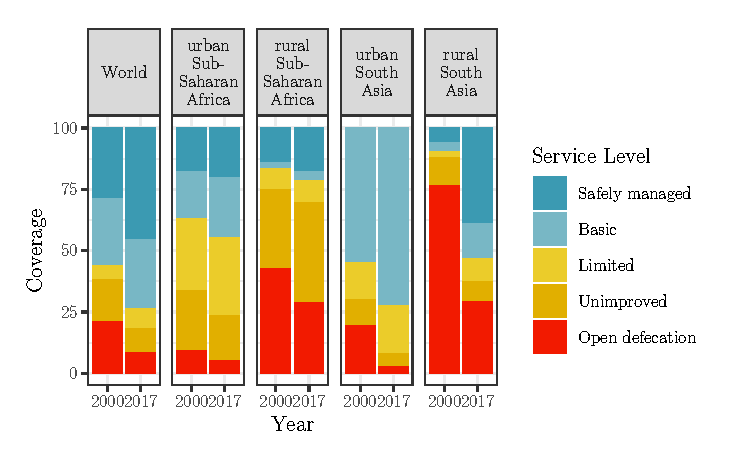
\includegraphics[width=\textwidth]{figures/coverage_plot.eps}
    \caption{Sanitation coverage 2000 and 2017 \citep{JMP2018}}
    \label{fig:coverage}
\end{figure}

Figure~\ref{fig:coverage} shows the evolution of sanitation coverage between 2000 and 2017 for the whole world and sub-Saharan Africa (SSA) based on data from the \cite{JMP2018}. The first panel shows that the coverage of basic and safely managed services has significantly improved across the world in the last two decades from 56\% to 74\%. Simultaneously, the share of the world's population practicing open defecation (OD) and using unimproved technologies decreased from 38\% to 18\%. However, limited sanitation (i.e., facilities with improved technologies, but shared by two or more households) actually increased from 5\% to 8\% over the same period and remained particularly high in urban areas of poor regions: In urban SSA, the share of limited sanitation was 31\% and in urban South Asia 19\%.

These statistics show that, first, preventing open defecation is not the main issue in urban areas of low- and middle-income countries anymore. Second, a large and increasing share of the urban population already has access to improved sanitation technologies, but they must share the toilet with other households. These two observations gain even more relevance considering that SSA and South Asia are often considered the world's fastest urbanizing regions. In 2017, 472 million people lived in urban areas in SSA, a figure projected to double over the next 25 years \citep{Lall2017}. In South Asia, the urban population is poised to rise by almost 250 million (or 50\%) to approximately 750 million by 2030 \citep{Ellis2015, TheWorldBank2020}. Hence, it is likely that many more toilets will be shared among multiple households in the future. Shared sanitation could be -- at least to date and given current technologies -- the only viable option for improving sanitation in urban low-income settlements \citep{Schouten2010}.

Therefore, the important question is whether we should continue labeling this sanitation solution as "limited" or if it can be labelled "adequate" under certain conditions. An  ill-defined  sanitation  service  ladder, that wrongly categorizes shared sanitation as inadequate, could have a dampening effect on policymakers’ incentive to allocate funds for shared sanitation leading to a misallocation of investments \citep{Evans2017}. In addition, ill-defined indicators could lead to misguided development objectives. Indicators for better education, for example, faced similar scrutiny. For a long time, enrollment rates were defined as indicators for better education (e.g., by the Millennium Development Goals), which led to a policy focus on achieving higher enrollment rates at the cost of quality. As a result, learning in schools stagnated or deteriorated in many countries \citep{WorldBank2018}.

In the literature, the JMP sanitation service ladder and whether its indicators are suited to measure "adequate" sanitation effectively is already contested \citep{Evans2017}. The main components of current JMP sanitation indicators -- toilet technology and the number of toilet users -- have been repeatedly challenged \citep{Mara2016, Evans2017}. For the case of technology, while observational studies tend to find large and robust effects of improved technologies on most child health variables \citep{Fink2011, Heijnen2014, Andres2017, Headey2019}, experimental studies show no effects on stunting and mixed-effects on diarrhea \citep{Clasen2014, Patil2015, Luby2018, Null2018, Humphrey2019}. 

The number of sharing users has not drawn as much scholarly attention. \cite{Tumwebaze2014, Tumwebaze2014a, Shiras2018} suggest that shared sanitation facilities are less likely to be clean than individual household toilets because of barriers to collective action to clean and maintain the toilet. Some empirical studies support this hypothesis and show that cleanliness deteriorates with an increasing number of users in Uganda and Kenya \citep{Gunther2012, Simiyu2017c}. In the case of Tanzania, on the other hand, \cite {Exley2015} find no correlation between shared toilets and pathogen contamination, relative to individual household toilets. However, it is fundamental to consider factors beyond hygiene, and associated health risks, in order to understand when shared sanitation is adequate for all users, such as privacy and safety, especially for women, children, and the elderly \citep{Gine-Garriga2017, Sclar2018, Kwiringira2014, Tidwell2018, Simiyu2017c, Schelbert2020}. 

One could hypothetically try to elicit the hygiene, privacy, and safety of a toilet using a household survey. In practice, the low reliability of reported data on sanitation quality outcomes prevents us from obtaining this information directly from respondents. At the same time, conducting observational spot-checks of toilet facilities is time consuming and expensive, and thus infeasible for large-scale surveys. 

This paper analyzes the correlation between observations of sanitation quality with various reported indicators that can be elicited in large-scale surveys and can be applied to determine whether a toilet facility is “adequate”. In particular, we first apply multivariate regression analysis to evaluate whether the current JMP indicators -- toilet technology and the number of users -- are of high relevance for a Sanitation Quality Index (SQI) composed of hygiene, safety, and privacy. In a second step, we test the correlation between sanitation quality and additional reported indicators that are likely to show low reporting bias. Examples are the toilet’s location, whether the toilet has a light, a bin, a lockable door, and whether there is a water source or a landlord living on the plot. We reconsider the current WHO/UNICEF Joint Monitoring Programme (JMP) framework and propose ways to improve it to measure access to adequate sanitation. 
%%%%%%%%%%%%%%%%%%%%%%%%%%%%%%%%%%%%%%%%%%%%%%%%
% Methods
%%%%%%%%%%%%%%%%%%%%%%%%%%%%%%%%%%%%%%%%%%%%%%%%
\section{Methods}
\label{sec:methods}
%
\subsection{Setting}
\label{sec:setting}
We conducted a cross-sectional study in low-income settlements between May and July 2019 in three cities: Kisumu, Kumasi, and Dhaka. Kisumu is the third largest city in Kenya, with a population of around 500,000 people \citep{KenyaNationalBureauofStatistics2019}. 47 percent of the population lives in low-income settlements \citep{NCPD2013}. Kumasi is Ghana's second-largest city, with a population of approximately 2.5 million people, an increasing share of whom are living in low-income settlements \citep{Amoako2011}. Dhaka is the capital of Bangladesh and the largest city in the country, with an estimated population of 20 million. Over a quarter of these people live in low-income settlements \citep{BangladeshBureauofStatistsics2019}. In all three cities, housing in low-income settlements is often organized in compounds, comprising several single-unit houses occupied by different households, most of whom are tenants. Households mostly share a toilet facility with others, which can have one or more cubicles. Operation and maintenance of these facilities is usually in the hands of the landlords or organized by the tenants, rather than outsourced to a paid cleaner \citep{Alam2017, Simiyu2017b, Antwi-Agyei2020}.
%
\FloatBarrier
%
\subsection{Sampling}
\label{sec:sampling}
The sampling strategy for the data collection consisted of three steps. First, between four and ten study areas were selected in each of the three cities based on income levels and the supposed prevalence of shared sanitation facilities. Only low-income areas with a prevalent use of shared sanitation facilities were eligible. Moreover, selected areas had to be distributed throughout the city. In a second step, up to four random geo-points were sampled in each study area using the geographic information software QGIS. The geo-points served as starting positions for the household sampling. Whenever possible, the (four) enumerators spread out in four different directions from the starting point. If there were fewer than four possible paths leading away from the point, the enumerators would walk in the same direction and split at the next opportunity (e.g., the next junction). In the third step, we applied a skipping pattern. The field assistants would start with the closest compound in the respective walking direction from the starting point, skipping the next two compounds and entering the third.\footnote{The terms compound and plot are used interchangeably in this paper.} Upon entering a compound, field assistants would interview two households if the respondents used a shared toilet and one household if it was a private toilet. Each household within a compound was assigned a number and randomly selected by drawing a number on a mobile phone application. The second household was identified by repeating the same procedure with the restriction that the second respondent had to use the same toilet cubicle as the first respondent. 

Respondents had to be at least 18 years of age, a resident of the compound (dwelling on the premises for at least three months), regularly using a shared/private/public toilet facility within walking distance, and voluntarily consent to participate in the study. If none of the respondents in a household met these criteria, the field assistants moved to the next available household on the compound. In most instances, enumerators interviewed the household head or the most knowledgeable person. Furthermore, if the respondent of the first household in the compound was a male, the enumerators aimed for a female respondent in the second interview and vice-versa.

Even though this study focuses on shared toilets, public and private toilets were still of interest for comparative purposes. We set the upper bound on the proportion of private and public toilets to not exceed 20\% within a given study area, ensuring a minimum of 80\% shared toilets in the total sample. Thus, the share of households using a private or public toilet is not representative for the chosen cities. Using the sampling described above, in Kenya and Bangladesh, we got too few households with individual household toilets for a meaningful analysis and, hence, had to use purposive sampling for individual household toilets.

Even though randomness within a given settlement was achieved through systematic sampling, the selection of settlements was purposive. We deliberately focused on settlements where the chance of encountering shared facilities was higher, following expert knowledge from our local partners. We tried to ensure a certain degree of geographic dispersion across cities, but middle- and high-income areas were deliberately excluded. Therefore, the distribution of sanitation outcomes does not represent the overall situation in each city, but only in specific low-income and middle-income settlements. As a consequence, respondent and toilet characteristics that are presumably associated with higher income areas are underrepresented. Moreover, middle- and high-income areas tend to have higher shares of private household toilets. Thus, the private toilets we encounter in low-income areas might not necessarily have the same characteristics as those encountered in middle- and high-income areas.
%
\FloatBarrier
%
\subsection{Data collection}
\label{sec:measures}

To analyze the role of self-reported, sanitation-related indicators in predicting observed sanitation quality outcomes, we relied on two primary data sources: the household survey questionnaire and spot-check observations of the toilet cubicles used by the interviewed households. Both potential quality outcomes and explanatory variables (candidate indicators) were identified through a combination of formative qualitative research and the WHO guidelines on sanitation \citep{Schelbert2020, WHO2018}.

The questionnaire was administered in person by trained field assistants. It was conducted in multiple local languages, and piloted extensively in the presence of the authors to ensure consistency across the three study sites. A detailed explanation for each variable used in this analysis is listed in Table~\ref{tab:variables} in Appendix~\ref{sec:variables}. In addition, the field assistants conducted spot-checks of toilets that respondents had indicated were their primary sanitation facility. The questionnaire and spot-check protocol can be found in \href{https://www.githubrepo.com}{Online Resource 1}.

Three sanitation quality dimensions were identified in focus group discussions as part of a formative qualitative study \citep{Schelbert2020}: hygiene, safety (and security), and privacy.\footnote{In contrast to the \cite{WHO2018} guidelines on sanitation and health, we do not include affordability and accessibility as quality dimensions. What is affordable depends on each individual's budget constraints and willingness to pay and is therefore not a suitable quality feature. Further, accessibility was excluded because it turned out to be covered by the other three dimensions and was not explicitly mentioned by participants during the focus group discussions.} For these three dimensions, the corresponding outcome variables were selected based on their relevance to the three quality dimensions and the feasibility of observing them during spot-checks. Due to concerns about the validity and reliability of reported cleanliness data, we focus exclusively on observable proxies for the quality outcomes (see Appendix~\ref{sec:reliability}). The quality dimensions and linked outcomes are:
\begin{itemize}
\item \textbf{Hygiene}: refers to intermediate cleanliness measures based on spot-check observations.
\begin{itemize}
    \item \textit{Solid waste} inside the cubicle
    \item \textit{Visible feces} in or around the manhole/pan
    \item \textit{Insects} inside the cubicle
    \item \emph{Handwashing facility \emph{with} soap}
    \item \textit{Clogged} in the case of a flush toilet or \textit{full} in the case of a pit latrine
\end{itemize}
\item \textbf{Safety}:
\begin{itemize}
    \item \textit{Solid roof (without holes)}: The roof protects the user from external (environmental) factors such as rain.
    \item \textit{Solid floor (without cracks/holes)}: The floor separates the user from excreta and is, therefore, a gatekeeper for health hazards through both direct contact and indirect contact, e.g., insects. A solid floor also prevents users, particularly children, from falling into the pit, should there be one. 
\end{itemize}
\item \textbf{Privacy}:
\begin{itemize}
    \item \textit{Solid wall}: The wall must be made out of solid material and have no holes that would allow a person to peek through.
\end{itemize}
\end{itemize}

To develop a single quality outcome measure, we aggregated the eight quality variables into a single index (see Section~\ref{sec:empirical}). 

\FloatBarrier

\subsection{Empirical Strategy}
\label{sec:empirical}
The empirical approach of this paper follows three steps. First, we calculate the Sanitation Quality Index (SQI) based on the three dimensions and eight variables described in the previous section. Second, we use regression analysis to study the relationship between the SQI, as a proxy for toilet quality, and currently used sanitation indicators, namely technology and sharing. Third we include additional candidate indicators in the regression analysis, that were identified as user quality priorities in \citet{Schelbert2020}. Fourth, we incorporate the findings into the current JMP framework to analyze the implications of new quality indicators for the sanitation service ladder.

Aggregating the eight observed quality variables into one single measure for toilet quality simplifies the analysis to a single outcome variable. \citet{Simiyu2017c} and \citet{Tidwell2018} provide similar examples of aggregated sanitation quality indices. \citet{Simiyu2017c} calculated a score with equal weights summed over 18 binary quality variables, each of which is assigned to one of three quality dimensions (hygiene, privacy, and toilet design). \citet{Tidwell2018} is guided by five quality dimensions -- hygiene, sustainability, use, desirability, and accessibility -- and assigns weights according to the number of variables within each quality category. Both methods have one caveat. The method applied by \citet{Simiyu2017c} implicitly gives more weight to dimensions that include more variables. Consequently, privacy, which includes eight variables, ends up having twice the weight of hygiene, which is only made up of four variables. The method applied by \citet{Tidwell2018} -- somewhat arbitrarily -- gives equal weight to each dimension.

Here, we propose to assign weights to the variables using Multiple Correspondence Analysis (MCA). MCA, a special case of Principal Component Analysis (PCA), allows for the analysis of patterns in the relationships between categorical dependent variables \citep{Abdi2007}. It accounts for the fact that one variable might provide more variation than others. This feature is generally desirable when constructing a measure that is supposed to capture differences between households. For example, PCA is used extensively to aggregate variables from questionnaires to develop wealth and socio-economic status indices based on household assets \citep{Filmer2001, McKenzie2005, Vyas2006}. 

MCA derives several orthogonal (i.e., uncorrelated) principal components equal to the number of variables used for the analysis. From the first principal component, weights are obtained, serving as statistical weights assigned to each variable. We aggregate the eight observed quality variables into a weighted average that provides us with a single quality score for each toilet cubicle. In the context of sanitation, the technique is based on the central assumption that the eight observed sanitation variables reflect an underlying variable, namely sanitation quality. The main advantage of this method is that the underlying variable accounts for the largest share of the variance and covariance in the data. Additionally, the statistical weights derived from MCA solve the problem of choosing arbitrary weights (see Appendix~\ref{sec:sqi} for a formal description of how the SQI is constructed.)

We subsequently use the SQI as a dependent variable in multivariate regressions to estimate the correlation between households' self-reported toilet indicators and observed and aggregated sanitation quality. The regressions are modeled using three different specifications. In the first model specification, toilet quality is regressed on the two indicators that currently determine the JMP sanitation service ladder, \textit{improved technology}\footnote{"Improved technology" refers to the definition by \cite{JMP2018}. Improved sanitation facilities include pit latrines with cement slabs and flush/pour-flush toilets draining to pits, septic tanks, and piped sewers.} and \textit{shared cubicle}:
\begin{equation}
\label{eq:reg1}
    SQI_{f} = \alpha_{if}+ \beta improved\_technology_{if} + \gamma shared\_cubicle_{if} + \delta_c +\varepsilon_{ifc},
\end{equation}
where $i$ represents a household, using facility $f$, in country $c$. The coefficient $\beta$ represents the difference in SQI scores between technologically improved and unimproved toilets holding the sharing status constant. Similarly, $\gamma$ represents the difference in SQI scores between shared and private toilets holding the toilet technology constant. The coefficient $\delta_c$ denotes a vector of country fixed effects, controlling for unobserved, but constant differences in SQI scores across countries. The error term, $\epsilon_{ifc}$, is clustered at the facility level accounting for correlated outcomes between two respondents using the same toilet. 

In the second specification, the two indicators, \textit{improved\_technology} and \textit{shared\_cubicle}, are decomposed into the categorical variables \textit{technology}, \textit{outflow}, and \textit{sharingHHs}. \textit{Technology} represents a dummy variable of technology category $J$: \textit{flush} (reference category), \textit{pit latrine (with slab)}, \textit{pit latrine (no slab)/other}. Similarly, \textit{outflow} denotes a dummy variable of categories $K$: \textit{piped sewer/septic tank} (reference category), \textit{pit}, and \textit{elsewhere}. \textit{SharingHH} denotes the number of households, $L$, sharing a cubicle, coded as a categorical variable.\footnote{The reason for using a categorical instead of a continuous variable is two-fold. First, it allows non-linear effects of the number of households on the SQI. Second, there is no specific data available for more than ten households, which would yield biased estimates if \textit{sharingHH} was treated as a continuous variable.} We estimate the following regression model:
\begin{multline}
\label{eq:reg2}
    SQI_{f} = \eta_{if} + \sum^{j\in J}\theta_{j} technology_{ifj} + \sum^{k\in K} \kappa_{k} outflow_{ifk} \\ 
    + \sum^{l\in L} \rho_{l} sharingHHs_{ifl} + \delta_c +\varepsilon_{ifc},
\end{multline}
where $\theta$, $\kappa$, and $\rho$ now represent regression coefficients corresponding to the category $J$, $K$, and $L$ of \textit{technology}, \textit{outflow} and \textit{sharingHHs}, respectively. Therefore, $\theta_{j}$, $\kappa_{k}$ and $\rho_{l}$ give us the difference in SQI scores between a category $j$ of $technology$, $outflow$, $sharingHHs$, and the omitted reference category. 

Finally, we add a list of additional candidate indicators $X_{if}$ to the regression model besides $technology$, $outflow$, and $sharingHHs$:\footnote{The additional indicators include: \textit{location}, \textit{water on premises}, \textit{handwashing facility with soap}, \textit{lighting}, \textit{lockable door}, \textit{tiling}, \textit{gender-separated cubicles}, \textit{cleaning arrangement}, \textit{user relationship}, \textit{age of toilet}, \textit{landlord on plot}, and \textit{bin inside cubicle}.}
\begin{multline}
\label{eq:reg3}
 SQI_{f} = \eta_{if} + \sum^{j\in J}\theta_{j} technology_{ifj} + \sum^{k\in K} \kappa_{k} outflow_{ifk} \\ 
    + \sum^{l\in L} \rho_{l} sharingHHs_{ifl} + \sum^{m \in M} \phi_{ifm} X_{ifm} + \delta_c +\varepsilon_{ifc},
\end{multline}
where $\phi_{ifm}$ provides us with marginal SQI difference in SQI scores in the presence of a toilet characteristic $k$, holding $technology$, $outflow$, $sharingHHs$, and all other variables constant. Equations~\ref{eq:reg1}, \ref{eq:reg2}, and~\ref{eq:reg3} are estimated for the pooled sample as well as separately for each country (in this case, $\delta_c$ is dropped from the regressions).

In a last step, these results are checked against the current JMP framework to analyze whether its currently used indicators for sanitation service levels are supported by the data. We assess the indicators’ performance at separating high-quality toilets from low-quality toilets -- as measured by the SQI. We compare different alternative sanitation service level specifications, where we manipulate the decisive criteria that classify sanitation facilities as basic, limited, or unimproved. 

\FloatBarrier
%%%%%%%%%%%%%%%%%%%%%%%%%%%%%%%%%%%%%%%%%%%%%%%%
% Results
%%%%%%%%%%%%%%%%%%%%%%%%%%%%%%%%%%%%%%%%%%%%%%%%
\section{Results}
\label{sec:results}

\subsection{Descriptive statistics}
\paragraph{Demographic characteristics.}
The sampling procedure yielded a sample size of 3,600 households, as reported in Table~\ref{tab:sampling}. The vast majority of respondents are female, possibly because women were more likely to be at home during the day when data were collected. Even though all study areas are poor urban settlements, household characteristics differ considerably across the three cities. Ghana, for example, has a considerably higher average household size than Kenya or Bangladesh.\footnote{For easier reading, the study sites are referred to by name of the country. Results from Kisumu will be referred to as results from Kenya, Kumasi as Ghana, and Dhaka as Bangladesh.} Meanwhile, Bangladesh has the highest number of household members per room: on average, a room is shared by 4.3 people in Bangladesh and 4.0 people in Ghana, while in Kenya it is shared by only 3.3 people. Bangladesh has the highest number of household heads without formal primary education (47\%), followed by Ghana (25\%), and Kenya (12\%). Home ownership is also distributed unevenly across the three country samples. In Kenya and Bangladesh, most respondents are informal tenants (76\% in Kenya and 84\% in Bangladesh), whereas in Ghana, a large share of respondents own the dwelling unit that they live in (49\%). This imbalance might be due to the large share of traditional compound housing in Kumasi (Ghana), where it is possible to have multiple housing unit owners per compound \citep{Tipple2011}.  

\begin{table}[ht]

\caption{\label{tab:sampling}Sample characteristics}
\centering
\resizebox{\linewidth}{!}{
\begin{tabular}[t]{lllll}
\toprule
Characteristic & Overall, N = 3,600 & Kenya, N = 1,229 & Ghana, N = 1,087 & Bangladesh, N = 1,284\\
\midrule
Respondent &  &  &  & \\
\hspace{1em}Second & 1,574 (44\%) & 539 (44\%) & 443 (41\%) & 592 (46\%)\\
\hspace{1em}First & 2,026 (56\%) & 690 (56\%) & 644 (59\%) & 692 (54\%)\\
Gender=female (respondent) & 2,833 (79\%) & 981 (80\%) & 837 (77\%) & 1,015 (79\%)\\
Gender=female (HH head) & 1,060 (29\%) & 332 (27\%) & 569 (52\%) & 159 (12\%)\\
HH size & 5.2 (2.3) & 5.0 (2.0) & 5.7 (3.1) & 5.0 (1.6)\\
HH members/room & 3.87 (2.13) & 3.25 (1.84) & 4.03 (2.80) & 4.33 (1.50)\\
Income (monthly, USD ppp) & 375 (320) & 211 (195) & 281 (346) & 544 (289)\\
Education (HH head) &  &  &  & \\
\hspace{1em}None & 1,020 (28\%) & 142 (12\%) & 269 (25\%) & 609 (47\%)\\
\hspace{1em}Primary & 1,271 (35\%) & 450 (37\%) & 246 (23\%) & 575 (45\%)\\
\hspace{1em}Secondary & 920 (26\%) & 433 (35\%) & 420 (39\%) & 67 (5.2\%)\\
\hspace{1em}Tertiary & 321 (8.9\%) & 159 (13\%) & 140 (13\%) & 22 (1.7\%)\\
\hspace{1em}Don't know & 68 (1.9\%) & 45 (3.7\%) & 12 (1.1\%) & 11 (0.9\%)\\
House ownership &  &  &  & \\
\hspace{1em}Owner & 926 (26\%) & 212 (17\%) & 535 (49\%) & 179 (14\%)\\
\hspace{1em}Free rent & 132 (3.7\%) & 27 (2.2\%) & 86 (7.9\%) & 19 (1.5\%)\\
\hspace{1em}Tenant (formal) & 454 (13\%) & 50 (4.1\%) & 395 (36\%) & 9 (0.7\%)\\
\hspace{1em}Tenant (informal) & 2,088 (58\%) & 940 (76\%) & 71 (6.5\%) & 1,077 (84\%)\\
Electricity & 3,489 (97\%) & 1,138 (93\%) & 1,073 (99\%) & 1,278 (100\%)\\
\bottomrule
\end{tabular}}
\end{table}
\FloatBarrier
\paragraph{Toilet characteristics (reported).}
Results in Table~\ref{tab:descriptive} indicate that toilet technologies are remarkably heterogeneous across the three study sites. In Kenya, the sampling procedure resulted in mostly pit latrines (with slab) (83\%), followed by flush to sewer/septic tank/pit (13\%). In Ghana, the sample is more equally distributed between flush to sewer/septic tank/pit (55\%) and pit latrines (with slab) (41\%). In Bangladesh, 90\% of all toilets flush to "elsewhere". For 52\% of those, the outflow is unknown to the respondent.\footnote{This finding reflects the fact that toilets in Dhaka are classified as "unimproved" following the JMP definition. Only about 10\% of toilets in Bangladesh would qualify as having "improved" toilet technology.} We further find that in Kenya (6.9) and Bangladesh (6.6), shared toilets have a considerably higher average number of households per toilet cubicle than in Ghana (5.98).\footnote{Individual household toilets are excluded here because their share is not representative due to the sampling procedure (see Section~\ref{sec:sampling}.)}

\begin{table}[ht]

\caption{\label{tab:descriptive}Reported toilet characteristics}
\centering
\begin{threeparttable}
\resizebox{\linewidth}{!}{
\begin{tabular}[t]{lllll}
\toprule
Characteristic & Overall, N = 3,600 & Kenya, N = 1,229 & Ghana, N = 1,087 & Bangladesh, N = 1,284\\
\midrule
Toilet technology &  &  &  & \\
\hspace{1em}Flush to sewer/septic/pit$^{\mathrm{a}}$ & 874 (24\%) & 161 (13\%) & 596 (55\%) & 117 (9.1\%)\\
\hspace{1em}Flush to elsewhere$^{\mathrm{abc}}$ & 1,174 (33\%) & 19 (1.5\%) & 3 (0.3\%) & 1,152 (90\%)\\
\hspace{1em}Pit latrine (with slab) & 1,479 (41\%) & 1,020 (83\%) & 448 (41\%) & 11 (0.9\%)\\
\hspace{1em}Pit latrine (no slab)/other & 73 (2.0\%) & 29 (2.4\%) & 40 (3.7\%) & 4 (0.3\%)\\
Sharing HHs/cubicle &  &  &  & \\
\hspace{1em}1 HH$^{\mathrm{d}}$ & 260 (7.2\%) & 73 (5.9\%) & 107 (9.8\%) & 80 (6.2\%)\\
\hspace{1em}2-4 HH & 1,105 (31\%) & 352 (29\%) & 374 (34\%) & 379 (30\%)\\
\hspace{1em}5-7 HH & 943 (26\%) & 294 (24\%) & 310 (29\%) & 339 (26\%)\\
\hspace{1em}8-10 HH & 652 (18\%) & 221 (18\%) & 164 (15\%) & 267 (21\%)\\
\hspace{1em}more than 10 HH & 640 (18\%) & 289 (24\%) & 132 (12\%) & 219 (17\%)\\
Location &  &  &  & \\
\hspace{1em}Inside dwelling & 220 (6.1\%) & 47 (3.8\%) & 98 (9.0\%) & 75 (5.8\%)\\
\hspace{1em}Inside compound/on plot & 3,251 (90\%) & 1,101 (90\%) & 970 (89\%) & 1,180 (92\%)\\
\hspace{1em}Elsewhere & 129 (3.6\%) & 81 (6.6\%) & 19 (1.7\%) & 29 (2.3\%)\\
Improved water on premises & 2,451 (68\%) & 455 (37\%) & 762 (70\%) & 1,234 (96\%)\\
Lighting & 1,455 (40\%) & 61 (5.0\%) & 612 (56\%) & 782 (61\%)\\
Lockable door &  &  &  & \\
\hspace{1em}No lock & 409 (11\%) & 259 (21\%) & 101 (9.3\%) & 49 (3.8\%)\\
\hspace{1em}Only inside & 478 (13\%) & 55 (4.5\%) & 58 (5.3\%) & 365 (28\%)\\
\hspace{1em}Only outside & 299 (8.3\%) & 190 (15\%) & 103 (9.5\%) & 6 (0.5\%)\\
\hspace{1em}Outside and inside & 2,414 (67\%) & 725 (59\%) & 825 (76\%) & 864 (67\%)\\
Tiling (floor) & 723 (20\%) & 74 (6.0\%) & 592 (54\%) & 57 (4.4\%)\\
Gender separated & 106 (2.9\%) & 5 (0.4\%) & 57 (5.2\%) & 44 (3.4\%)\\
Cleaning rota & 1,541 (43\%) & 169 (14\%) & 486 (45\%) & 886 (69\%)\\
User relationship &  &  &  & \\
\hspace{1em}Only relatives & 294 (8.2\%) & 87 (7.1\%) & 127 (12\%) & 80 (6.2\%)\\
\hspace{1em}Close neighbors/landlord & 469 (13\%) & 304 (25\%) & 141 (13\%) & 24 (1.9\%)\\
\hspace{1em}Other tenants/unknown & 2,837 (79\%) & 838 (68\%) & 819 (75\%) & 1,180 (92\%)\\
Age of toilet &  &  &  & \\
\hspace{1em}less than 1 year & 434 (12\%) & 195 (16\%) & 54 (5.0\%) & 185 (14\%)\\
\hspace{1em}1-3 years & 955 (27\%) & 459 (37\%) & 193 (18\%) & 303 (24\%)\\
\hspace{1em}4-6 years & 597 (17\%) & 253 (21\%) & 126 (12\%) & 218 (17\%)\\
\hspace{1em}7-9 years & 238 (6.6\%) & 63 (5.1\%) & 77 (7.1\%) & 98 (7.6\%)\\
\hspace{1em}more than 9 years/don't know & 1,376 (38\%) & 259 (21\%) & 637 (59\%) & 480 (37\%)\\
Landlord on plot & 1,874 (52\%) & 456 (37\%) & 956 (88\%) & 462 (36\%)\\
Bin inside cubicle & 389 (11\%) & 1 (<0.1\%) & 377 (35\%) & 11 (0.9\%)\\
\bottomrule
\end{tabular}}
\begin{tablenotes}
\item[a] Flush includes both flush and pour-flush;
\item[b] Flush to elsewhere contains both flush to don’t know where as well as flush to open drain; 
\item[c] We assume toilets draining elsewhere involve an unsafe conveyance system;
\item[d] The share of households using private toilets is not representative for the samples as these households\newline(and toilets) were purposively sampled.
\end{tablenotes}
\end{threeparttable}
\end{table}

The toilets' location is relatively equally distributed across country samples. Most toilets are located outside of the individual dwelling, but within the compound (90\%). In total, 68\% report having access to an improved water source on their premises. Only a fraction of respondents report having lighting inside the toilet cubicle in Kenya (5\%), as opposed to Ghana (56\%) and Bangladesh (61\%). Most cubicles are lockable either from the inside or the outside; 67\% are both. In Kenya and Ghana, more toilets exhibit an outside lock (Kenya 74\%; Ghana 85\%) than an inside lock (Kenya 63\%; Ghana 81\%), whereas, in Bangladesh, almost all toilets have an inside lock (96\%) and fewer have an outside lock (68\%). In terms of floor tiling, Ghana stands out with 54\% compared to 6\% in Kenya and 4\% in Bangladesh. 

The share of gender-separated toilets is below 5\% throughout. Compared to the other two countries, few respondents in Kenya report having a cleaning rota (Kenya 14\%; Ghana 45\%; Bangladesh 69\%). The term, "user relationship," describes the social proximity between the respondent's household and the other users. The majority of toilets are used only by relatives and close neighbors, except for Ghana, where 19\% report that the toilet is also shared among individuals who are not next-door neighbors and people from outside the compound. In Ghana, toilets are older than in the other two countries -- 59\% reported that the toilet was built ten or more years ago.\footnote{In case the respondent did not know, the length of time the respondent lived on the plot was applied.} There is also an exceptionally high share of landlords or caretakers in Ghana that live in the same compound as the respondent (88\% compared to 37\% in Kenya and 36\% in Bangladesh). In Ghana, bins for solid waste are frequently found inside the toilet cubicle (59\%).\footnote{The share of bins outside the cubicle is very low in all three countries.} In contrast, in Kenya and Bangladesh, the share is below 1\% and 2\%, respectively.

Hence, the toilet technology as well as other toilet characteristics seem to vary widely across countries, which might lead to differences in sanitation quality. We were therefore not able to analyze challenges that are associated with a specific type of toilet technology across all three countries. For example, emptying arrangements are most certainly an essential factor for the quality of pit latrines, but could not be studied in this cross-country context.

\FloatBarrier
%%%%%%%%%%%%%%%%%%%%%%%%%%%%%%%%%%%%%%%%%%%%%%%%%%%%%%%%%%
\paragraph{Sanitation Quality Index -- SQI (observed).}
Figure~\ref{fig:sqi} shows the distribution of SQI scores for each city. The first panel shows the SQI scores resulting from a pooled Multiple Correspondence Analysis (MCA), where observations from all three countries (cities) are included in calculating the index weights. The second panel relies on an MCA computed separately for each country (city). All observations are binned according to their SQI score in equal bins of 20 points on the SQI scale. Overall, we find that most of the observations end up having a score between 60 and 100, indicating a skewed distribution of scores. On average, the toilets in Kenya have the lowest SQI scores out of all three countries. In the first panel, 40\% of toilets in Kenya have a SQI score of 80 or below. In Ghana, less than 6\% of toilets have SQI scores of 60 and below, and in Bangladesh, approximately 12\% fall below a score of 60. Compared to the pooled SQI, the SQI score by country tends to have more variation. This difference is particularly striking in Ghana.

\begin{figure}[htbp]
    \centering
    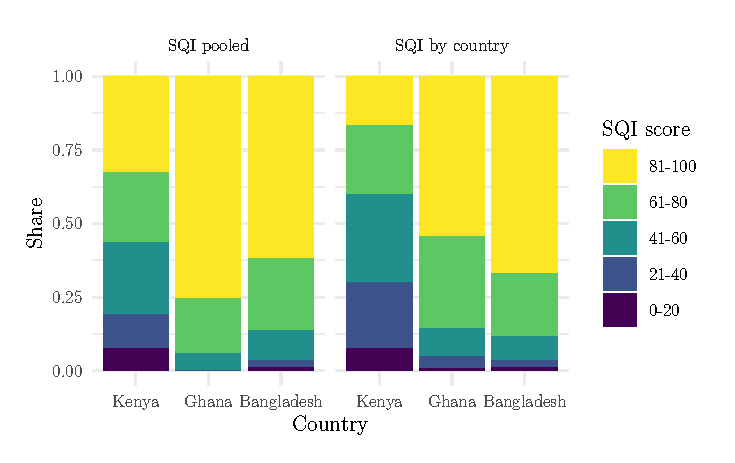
\includegraphics[width=0.9\textwidth]{figures/sqi_ctry.eps}
    \caption{Distribution of SQI scores by country}
    \label{fig:sqi}
\end{figure}

Table~\ref{tab:outcomes} shows the observed toilet quality variables that were used to construct the SQI. A more detailed description of the variables can be found in Appendix~\ref{sec:variables}. We see that all dimensions of the SQI drive the uneven SQI distribution, i.e., cleanliness, safety, and privacy, in which Kenyan toilets consistently score lower than toilets in Bangladesh and Ghana. Only 21\% of shared urban toilets in Kenya are clean, measured as neither insects nor visible feces nor solid waste being observed, followed by Bangladesh (43\%), and Ghana (61\%). There is also a high divergence in full and clogged toilets. In Kenya, in more than a third of the cases, the toilet's pit was full or the toilet was clogged. This observation stands in contrast to just over 8\% in Ghana and 6\% in Bangladesh. Handwashing facilities with soap are absent in all but 11\% of the toilet facilities. The share is lowest in Kenya (2\%), followed by Ghana (10\%), and Bangladesh (22\%). 
\begin{table}[ht]

\caption{\label{tab:outcomes}Toilet quality outcomes (observed)}
\centering
\begin{threeparttable}
\resizebox{\linewidth}{!}{
\begin{tabular}[t]{lllll}
\toprule
Characteristic & Overall, N = 3,600 & Kenya, N = 1,229 & Ghana, N = 1,087 & Bangladesh, N = 1,284\\
\midrule
Pooled SQI & 75.2 (21.7) & 62.0 (25.0) & 85.1 (12.7) & 79.3 (18.0)\\
Country SQI & 70.5 (23.5) & 53.0 (22.4) & 75.5 (17.3) & 83.0 (18.4)\\
Toilet clean (composite) & 1,470 (41\%) & 261 (21\%) & 662 (61\%) & 547 (43\%)\\
Visible feces & 807 (22\%) & 450 (37\%) & 89 (8.2\%) & 268 (21\%)\\
Insects & 1,532 (43\%) & 875 (71\%) & 226 (21\%) & 431 (34\%)\\
Solid waste & 1,158 (32\%) & 522 (42\%) & 233 (21\%) & 403 (31\%)\\
Toilet full or clogged & 584 (16\%) & 419 (34\%) & 92 (8.5\%) & 73 (5.7\%)\\
Wall material (high quality) & 3,193 (89\%) & 1,032 (84\%) & 1,041 (96\%) & 1,120 (87\%)\\
Floor material (high quality) & 3,280 (91\%) & 1,024 (83\%) & 1,057 (97\%) & 1,199 (93\%)\\
Roof material (high quality) & 2,832 (79\%) & 790 (64\%) & 982 (90\%) & 1,060 (83\%)\\
Handwashing station (with soap) & 413 (11\%) & 23 (1.9\%) & 105 (9.7\%) & 285 (22\%)\\
\bottomrule
\end{tabular}}
\begin{tablenotes}
\item[a] The toilet is considered clean if no visible feces, insects, and solid waste were observed.
\end{tablenotes}
\end{threeparttable}
\end{table}

\FloatBarrier

%%%%%%%%%%%%%%%%%%%%%%%%%%%%%%%%%%%%%%%%%%%%%%%%%%%%%%%%%%
\subsection{Regression results: technology and number of households}

To test whether technology, the number of households, and potential alternative indicators are good predictors of sanitation quality (as measured by the SQI), we compare different models of multivariate linear regressions. In all subsequent regression tables, we report robust standard errors clustered at the compound level because of the sampling strategy (see Section~\ref{sec:sampling}. While some of the variables are household-level data from the questionnaire, other variables are compound-level data, in particular those based on the spot-check observation. Using clustered standard errors, we acknowledge that the residuals may be correlated for respondents dwelling on the same compound. Additionally, all regressions on the pooled sample include country fixed effects to control for constant, but unobserved differences in SQI scores between countries.

Table~\ref{tab:reg_current} reports the regression results for the correlation between technology and number of sharing households. The results in columns 1-4 correspond to equation~\ref{eq:reg1} in Section~\ref{sec:empirical}. The explanatory variables, improved technology and whether a toilet is shared by two or more households, are the two indicators currently used by WHO/UNICEF for the sanitation service level assessment. On average, the SQI scores of technologically improved toilets -- defined as pit latrines with a cement slab or flush/pour-flush to piped sewers/septic tanks/pits by WHO/UNICEF -- are not statistically different from unimproved toilets. In none of the country-specific regressions do we find a significant difference in SQI scores between "improved" and "unimproved" technology as defined by WHO/UNICEF. For Bangladesh, this result is driven by toilets being classified as unimproved due to the outflow and not the interface. In Kenya and Ghana, the difference is sizable, but insignificant due to a small share of toilets that classify as unimproved according to WHO/UNICEF (see Table~\ref{tab:descriptive}). 

\begin{table}
\caption{OLS regression results of SQI on common indicators}
\center
\resizebox{\textwidth}{!}{

\begin{threeparttable}
\begin{tabular}{l@{} c@{} c@{} c@{} c@{} c@{} c@{} c@{} c@{}}
\toprule
 & \multicolumn{1}{c}{Pooled SQI} & \multicolumn{3}{c}{Country SQI} & \multicolumn{1}{c}{Pooled SQI} & \multicolumn{3}{c}{Country SQI} \\
\cmidrule(lr){2-2} \cmidrule(lr){3-5} \cmidrule(lr){6-6} \cmidrule(lr){7-9}
 & All & Kenya & Ghana & Bangladesh & All & Kenya & Ghana & Bangladesh \\
\midrule
Improved technology (ref=\textit{No})          & $2.40$         & $5.36$         & $4.25$        & $-0.43$       &                &                &                &                \\
                                               & $(1.99)$       & $(5.02)$       & $(3.26)$      & $(2.42)$      &                &                &                &                \\
Shared cubicle (ref=\textit{No})               & $-12.29^{***}$ & $-26.30^{***}$ & $-9.24^{***}$ & $-4.03^{*}$   &                &                &                &                \\
                                               & $(1.04)$       & $(2.27)$       & $(1.70)$      & $(1.89)$      &                &                &                &                \\
Technology (ref=\textit{Flush})                &                &                &               &               &                &                &                &                \\
                                               &                &                &               &               &                &                &                &                \\
\quad Pit latrine (with slab)                  &                &                &               &               & $-14.68^{***}$ & $-18.01^{***}$ & $-2.16$        &                \\
                                               &                &                &               &               & $(2.64)$       & $(2.92)$       & $(4.79)$       &                \\
\quad Pit latrine (no slab)/other              &                &                &               &               & $-24.66^{***}$ & $-39.14^{***}$ & $1.99$         & $-43.31^{***}$ \\
                                               &                &                &               &               & $(4.33)$       & $(5.57)$       & $(5.33)$       & $(12.98)$      \\
Outflow (ref=\textit{Piped sewer/septic tank}) &                &                &               &               &                &                &                &                \\
                                               &                &                &               &               &                &                &                &                \\
\quad Pit                                      &                &                &               &               & $-0.40$        & $-7.32^{*}$    & $-10.38^{*}$   & $-8.59$        \\
                                               &                &                &               &               & $(2.61)$       & $(3.23)$       & $(4.68)$       & $(8.59)$       \\
\quad Elsewhere                                &                &                &               &               & $1.46$         & $-1.30$        & $-13.64^{*}$   & $-4.41^{*}$    \\
                                               &                &                &               &               & $(1.79)$       & $(3.27)$       & $(6.86)$       & $(1.77)$       \\
Sharing HHs (ref=\textit{1 HH})                &                &                &               &               &                &                &                &                \\
                                               &                &                &               &               &                &                &                &                \\
\quad 2 HH                                     &                &                &               &               & $-6.16^{***}$  & $-7.65^{**}$   & $-2.92$        & $-5.30$        \\
                                               &                &                &               &               & $(1.57)$       & $(2.77)$       & $(2.12)$       & $(3.48)$       \\
\quad 3 HH                                     &                &                &               &               & $-6.10^{***}$  & $-8.18^{**}$   & $-7.47^{**}$   & $-0.24$        \\
                                               &                &                &               &               & $(1.42)$       & $(2.65)$       & $(2.45)$       & $(2.74)$       \\
\quad 4 HH                                     &                &                &               &               & $-9.78^{***}$  & $-13.19^{***}$ & $-7.38^{**}$   & $-5.79^{*}$    \\
                                               &                &                &               &               & $(1.48)$       & $(2.72)$       & $(2.25)$       & $(2.92)$       \\
\quad 5 HH                                     &                &                &               &               & $-9.68^{***}$  & $-12.93^{***}$ & $-8.87^{***}$  & $-2.61$        \\
                                               &                &                &               &               & $(1.46)$       & $(3.01)$       & $(2.21)$       & $(2.71)$       \\
\quad 6 HH                                     &                &                &               &               & $-9.43^{***}$  & $-14.87^{***}$ & $-8.50^{***}$  & $-2.41$        \\
                                               &                &                &               &               & $(1.38)$       & $(2.73)$       & $(2.27)$       & $(2.47)$       \\
\quad 7 HH                                     &                &                &               &               & $-8.85^{***}$  & $-11.79^{***}$ & $-10.92^{***}$ & $-1.20$        \\
                                               &                &                &               &               & $(1.65)$       & $(2.81)$       & $(2.98)$       & $(2.68)$       \\
\quad 8 HH                                     &                &                &               &               & $-10.69^{***}$ & $-19.15^{***}$ & $-6.37^{*}$    & $-1.51$        \\
                                               &                &                &               &               & $(1.79)$       & $(3.63)$       & $(3.02)$       & $(2.64)$       \\
\quad 9 HH                                     &                &                &               &               & $-9.47^{***}$  & $-15.17^{***}$ & $-6.10$        & $-2.63$        \\
                                               &                &                &               &               & $(2.19)$       & $(4.10)$       & $(3.48)$       & $(3.38)$       \\
\quad 10 HH                                    &                &                &               &               & $-12.94^{***}$ & $-18.13^{***}$ & $-9.43^{**}$   & $-6.93$        \\
                                               &                &                &               &               & $(2.16)$       & $(3.85)$       & $(3.01)$       & $(3.71)$       \\
\quad $>$10 HH                                 &                &                &               &               & $-15.03^{***}$ & $-21.80^{***}$ & $-11.18^{***}$ & $-7.34^{**}$   \\
                                               &                &                &               &               & $(1.31)$       & $(2.20)$       & $(2.42)$       & $(2.35)$       \\
Ghana FE                                       & $22.58^{***}$  &                &               &               & $15.90^{***}$  &                &                &                \\
                                               & $(1.09)$       &                &               &               & $(1.12)$       &                &                &                \\
Bangladesh FE                                  & $19.31^{***}$  &                &               &               & $2.63$         &                &                &                \\
                                               & $(2.17)$       &                &               &               & $(2.08)$       &                &                &                \\
(Intercept)                                    & $71.29^{***}$  & $72.58^{***}$  & $79.79^{***}$ & $86.86^{***}$ & $85.03^{***}$  & $89.83^{***}$  & $88.40^{***}$  & $91.21^{***}$  \\
                                               & $(2.25)$       & $(5.32)$       & $(3.34)$      & $(1.72)$      & $(1.27)$       & $(1.58)$       & $(1.46)$       & $(2.44)$       \\
\midrule
R$^2$                                          & $0.22$         & $0.08$         & $0.03$        & $0.00$        & $0.31$         & $0.27$         & $0.18$         & $0.10$         \\
Adj. R$^2$                                     & $0.22$         & $0.08$         & $0.02$        & $0.00$        & $0.31$         & $0.26$         & $0.17$         & $0.09$         \\
Num. obs.                                      & $3600$         & $1229$         & $1087$        & $1284$        & $3600$         & $1229$         & $1087$         & $1284$         \\
N Clusters                                     & $2013$         & $687$          & $633$         & $693$         & $2013$         & $687$          & $633$          & $693$          \\
\bottomrule
\end{tabular}
\begin{tablenotes}[flushleft]
\scriptsize{\item[\hspace{-5mm}] Standard errors are clustered on the compound level; \item[\hspace{-5mm}] All pooled regressions include country fixed effects; \item[\hspace{-5mm}] $^{***}p<0.001$; $^{**}p<0.01$; $^{*}p<0.05$.}
\end{tablenotes}
\end{threeparttable}

}
\label{tab:reg_current}
\end{table}

The coefficient for a shared toilet cubicle is negative and statistically significant for the pooled sample (Table~\ref{tab:reg_current}, Col.1). On average, the SQI of shared cubicles is 12 points below private toilets, which show an SQI of 74.1 on average. The negative coefficient for toilet sharing is particularly evident for the Kenyan sample. On average, shared facilities are 26 SQI points below facilities that are used by only one household. In Ghana, shared toilets score 9 points lower than private toilets, and only 4 points lower in Bangladesh. These results suggest that improved sanitation technology (as currently defined) is generally not associated with toilet quality, and for shared cubicles the magnitude of the effect is highly context sensitive.

The results in Table~\ref{tab:reg_current}, Cols.5-8 show the impact of technology, outflow, and number of sharing households as categorical variables (see equation~\ref{eq:reg2}). Results indicate that for the pooled sample, SQI scores of improved pit latrines (with slab) are more than 14 points lower than those of flush toilets (even though both are categorized as improved by the current WHO/UNICEF definition). The SQI of pit latrines with no slab and other technologies is on average 24 points lower than flush toilets.\footnote{Other toilet types include container based sanitation, composting toilets without cements slab, and hanging latrines.} This result is mainly driven by the Kenyan sample. In Ghana, the difference in toilet types is much more driven by the outflow (piped sewer/septic tank vs. pit vs. elsewhere) than by the interface technology. In Bangladesh, the sample consists of mostly pour-flush toilets, making a comparison to other technologies unreliable. 

The number of sharing households is negatively correlated with toilet quality, but the results suggest that the relationship between the number of sharing households and the SQI score is not linear. Based on the pooled sample, there appears to be a large gap between one and two households, and no significant difference between two and three households. There is again a moderate difference between three and four households, whereas between four and nine households, average SQI scores stay relatively constant and only increase again with ten households or more. These results are again mainly driven by Kenyan households, whereas the differences are less pronounced in Ghana. Interestingly, the number of sharing households does not provide any conclusions on toilet quality in Bangladesh: only toilets that are shared by more than ten households tend to be of lower quality.

%%%%%%%%%%%%%%%%%%%%%%%%%%%%%%%%%%%%%%%%%%%%%%%%%%%%
\subsection{Regression results: additional variables}

In Table~\ref{tab:reg_all}, various potential indicators for sanitation quality are included (see equation~\ref{eq:reg3}). The overall results show that the magnitude of the coefficients for technology and sharing households decreases considerably. In Kenya, this has the consequence that the coefficients for 2 and 3 households are no longer significant. In Ghana and Bangladesh, the consequence is that any number of households is no longer a significant predictor of toilet quality. This means that some of the added variables are correlated with the number of sharing households and the SQI.


\begin{center}
\begin{scriptsize}
\begin{ThreePartTable}
\begin{TableNotes}[flushleft]
\tiny{\item[\hspace{-5mm}] Standard errors are clustered on the compound level. \item[\hspace{-5mm}] All pooled regressions include country fixed effects. \item[\hspace{-5mm}] $^{***}p<0.001$; $^{**}p<0.01$; $^{*}p<0.05$.}
\end{TableNotes}
\begin{longtable}{l@{} c@{} c@{} c@{} c@{}}
\caption{OLS regression results of SQI on common and alternative indicators}
\label{tab:reg_all}\\
\toprule
 & \multicolumn{1}{c}{Pooled SQI} & \multicolumn{3}{c}{Country SQI} \\
\cmidrule(lr){2-2} \cmidrule(lr){3-5}
 & All & Kenya & Ghana & Bangladesh \\
\midrule
\endfirsthead
\toprule
 & \multicolumn{1}{c}{Pooled SQI} & \multicolumn{3}{c}{Country SQI} \\
\cmidrule(lr){2-2} \cmidrule(lr){3-5}
 & All & Kenya & Ghana & Bangladesh \\
\midrule
\endhead
\bottomrule
\endfoot
\bottomrule
\insertTableNotes\\
\endlastfoot
Technology (ref=\textit{Flush})                            &                &                &               &               \\
                                                           &                &                &               &               \\
\quad Pit latrine (with slab)                              & $-11.09^{***}$ & $-13.30^{***}$ & $-3.24$       &               \\
                                                           & $(2.27)$       & $(2.69)$       & $(4.49)$      &               \\
\quad Pit latrine (no slab)/other                          & $-17.59^{***}$ & $-28.44^{***}$ & $2.54$        & $-28.68^{*}$  \\
                                                           & $(3.82)$       & $(5.46)$       & $(5.05)$      & $(12.62)$     \\
Outflow (ref=\textit{Piped sewer/septic tank})             &                &                &               &               \\
                                                           &                &                &               &               \\
\quad Pit                                                  & $-0.69$        & $-6.74^{*}$    & $-7.51$       & $-5.75$       \\
                                                           & $(2.24)$       & $(2.96)$       & $(4.39)$      & $(7.36)$      \\
\quad Elsewhere                                            & $0.48$         & $-1.46$        & $-10.58$      & $-4.15^{**}$  \\
                                                           & $(1.58)$       & $(2.71)$       & $(6.45)$      & $(1.57)$      \\
Sharing HHs (ref=\textit{1 HH})                            &                &                &               &               \\
                                                           &                &                &               &               \\
\quad 2 HH                                                 & $-4.09^{*}$    & $-5.96$        & $0.92$        & $-9.43$       \\
                                                           & $(1.83)$       & $(3.04)$       & $(2.52)$      & $(6.56)$      \\
\quad 3 HH                                                 & $-4.20^{*}$    & $-5.83$        & $-1.69$       & $-5.94$       \\
                                                           & $(1.91)$       & $(3.14)$       & $(2.57)$      & $(6.81)$      \\
\quad 4 HH                                                 & $-7.56^{***}$  & $-10.34^{**}$  & $-1.75$       & $-9.93$       \\
                                                           & $(1.91)$       & $(3.15)$       & $(2.62)$      & $(6.98)$      \\
\quad 5 HH                                                 & $-7.62^{***}$  & $-11.01^{**}$  & $-3.76$       & $-6.04$       \\
                                                           & $(1.93)$       & $(3.40)$       & $(2.52)$      & $(6.85)$      \\
\quad 6 HH                                                 & $-7.02^{***}$  & $-10.77^{**}$  & $-3.51$       & $-6.66$       \\
                                                           & $(1.98)$       & $(3.56)$       & $(2.63)$      & $(6.87)$      \\
\quad 7 HH                                                 & $-6.20^{**}$   & $-7.28^{*}$    & $-3.64$       & $-6.76$       \\
                                                           & $(2.08)$       & $(3.31)$       & $(3.22)$      & $(6.78)$      \\
\quad 8 HH                                                 & $-7.88^{***}$  & $-12.97^{***}$ & $-1.75$       & $-5.30$       \\
                                                           & $(2.14)$       & $(3.76)$       & $(3.22)$      & $(6.89)$      \\
\quad 9 HH                                                 & $-7.11^{**}$   & $-10.44^{**}$  & $-2.32$       & $-7.23$       \\
                                                           & $(2.40)$       & $(3.85)$       & $(3.65)$      & $(7.10)$      \\
\quad 10 HH                                                & $-10.15^{***}$ & $-13.03^{**}$  & $-4.66$       & $-11.46$      \\
                                                           & $(2.50)$       & $(4.05)$       & $(3.55)$      & $(7.34)$      \\
\quad $>$10 HH                                             & $-11.06^{***}$ & $-15.92^{***}$ & $-5.55$       & $-9.40$       \\
                                                           & $(1.89)$       & $(2.88)$       & $(3.01)$      & $(6.69)$      \\
Location (ref=\textit{Inside dwelling})                    &                &                &               &               \\
                                                           &                &                &               &               \\
\quad Inside compound                                      & $-1.39$        & $0.56$         & $-7.94^{***}$ & $5.05$        \\
                                                           & $(1.36)$       & $(3.10)$       & $(1.57)$      & $(4.04)$      \\
\quad Outside compound                                     & $-11.06^{***}$ & $-8.18^{*}$    & $-7.96^{*}$   & $-6.73$       \\
                                                           & $(2.63)$       & $(3.92)$       & $(3.27)$      & $(6.50)$      \\
Water on premises (ref=\textit{No})                        & $2.05^{*}$     & $2.86^{*}$     & $-0.81$       & $4.05$        \\
                                                           & $(1.01)$       & $(1.42)$       & $(1.44)$      & $(4.32)$      \\
Lighting (ref=\textit{No})                                 & $3.87^{***}$   & $2.51$         & $3.79^{**}$   & $5.90^{***}$  \\
                                                           & $(0.84)$       & $(2.66)$       & $(1.30)$      & $(1.40)$      \\
Lockable door (ref=\textit{Not lockable})                  &                &                &               &               \\
                                                           &                &                &               &               \\
\quad Only inside                                          & $9.63^{***}$   & $10.19^{**}$   & $0.44$        & $10.75^{*}$   \\
                                                           & $(1.85)$       & $(3.44)$       & $(3.03)$      & $(4.64)$      \\
\quad Only outside                                         & $9.55^{***}$   & $10.34^{***}$  & $-1.53$       & $5.31$        \\
                                                           & $(1.99)$       & $(2.36)$       & $(2.99)$      & $(9.70)$      \\
\quad Outside and inside                                   & $15.75^{***}$  & $16.67^{***}$  & $2.83$        & $16.82^{***}$ \\
                                                           & $(1.48)$       & $(1.87)$       & $(2.09)$      & $(4.43)$      \\
Tiling (ref=\textit{No})                                   & $4.14^{***}$   & $6.48^{**}$    & $6.16^{***}$  & $3.63$        \\
                                                           & $(0.92)$       & $(2.00)$       & $(1.39)$      & $(2.23)$      \\
Gender separated (ref=\textit{No})                         & $1.52$         & $1.81$         & $2.58$        & $-1.80$       \\
                                                           & $(1.72)$       & $(7.57)$       & $(2.46)$      & $(3.10)$      \\
Cleaning rota (ref=\textit{No})                            & $4.23^{***}$   & $2.28$         & $2.83^{*}$    & $4.70^{**}$   \\
                                                           & $(0.85)$       & $(1.82)$       & $(1.39)$      & $(1.58)$      \\
User relationship (ref=\textit{Relatives/close neighbors}) &                &                &               &               \\
                                                           &                &                &               &               \\
\quad Other tenants/unknown                                & $-2.37$        & $-3.80^{*}$    & $-2.20$       & $-0.72$       \\
                                                           & $(1.21)$       & $(1.63)$       & $(1.59)$      & $(4.67)$      \\
Toilet age, years (ref=\textit{$<$1})                      &                &                &               &               \\
                                                           &                &                &               &               \\
\quad 1-3                                                  & $-0.65$        & $0.82$         & $-0.20$       & $-2.34$       \\
                                                           & $(1.10)$       & $(1.60)$       & $(2.61)$      & $(1.63)$      \\
\quad 4-6                                                  & $0.41$         & $1.12$         & $1.53$        & $-1.19$       \\
                                                           & $(1.23)$       & $(1.81)$       & $(2.77)$      & $(1.84)$      \\
\quad 7-9                                                  & $-0.43$        & $-2.48$        & $6.42^{*}$    & $-0.66$       \\
                                                           & $(1.50)$       & $(2.61)$       & $(2.61)$      & $(2.44)$      \\
\quad $>$9                                                 & $-1.89$        & $-2.83$        & $1.35$        & $-2.18$       \\
                                                           & $(1.10)$       & $(1.93)$       & $(2.41)$      & $(1.58)$      \\
Landlord on plot (ref=\textit{No})                         & $-0.97$        & $-1.28$        & $0.58$        & $-1.09$       \\
                                                           & $(0.88)$       & $(1.34)$       & $(1.80)$      & $(1.36)$      \\
Bin inside cubicle (ref=\textit{No})                       & $-1.35^{*}$    & $4.81^{*}$     & $-1.11$       & $2.34$        \\
                                                           & $(0.67)$       & $(2.18)$       & $(0.81)$      & $(2.39)$      \\
Ghana FE                                                   & $10.47^{***}$  &                &               &               \\
                                                           & $(1.29)$       &                &               &               \\
Bangladesh FE                                              & $-1.07$        &                &               &               \\
                                                           & $(2.03)$       &                &               &               \\
(Intercept)                                                & $71.14^{***}$  & $70.78^{***}$  & $81.79^{***}$ & $67.46^{***}$ \\
                                                           & $(2.26)$       & $(3.80)$       & $(4.03)$      & $(6.87)$      \\
\midrule
R$^2$                                                      & $0.40$         & $0.39$         & $0.26$        & $0.22$        \\
Adj. R$^2$                                                 & $0.40$         & $0.38$         & $0.24$        & $0.20$        \\
Num. obs.                                                  & $3600$         & $1229$         & $1087$        & $1284$        \\
N Clusters                                                 & $2013$         & $687$          & $633$         & $693$         \\
\end{longtable}
\end{ThreePartTable}
\end{scriptsize}
\end{center}


Apart from the technology and the number of sharing households, the results suggest that the location affects SQI scores. Toilets located outside of the compound have, on average, an SQI score that is 11 points lower than toilets inside the compound. Moreover, the results suggest that a lockable door is positively associated with SQI scores. Having the option to lock the door from the inside and the outside improves the SQI score by 16 points. Having the option to lock the door only from the inside or only from the outside improves the SQI score by more than 10 points. Other features that show a moderate positive correlation with toilet quality are lighting, floor tiling, and cleaning rotas. The availability of water on the premises, gender-separated cubicles, the relationship between the users, the age of the toilet, whether there is a landlord residing on the same plot, and a bin inside the cubicle are not significantly associated with SQI scores. 

In addition to the regressions in Tables~\ref{tab:reg_current} and \ref{tab:reg_all}, where the SQI is the dependent variable, Table~\ref{tab:reg_add_ctry} in  Appendix~\ref{sec:robustness} reports the results for a robustness check using an additive sanitation quality measure. In this specification, the eight toilet quality features that constitute the SQI are weighted equally, and the score takes values between one and eight. Results remain qualitatively unchanged due to the high correlation between the SQI and the alternative additive quality score (see Figure~\ref{fig:corr_additive} in Appendix~\ref{sec:robustness}).

Comparing the $R^2$ statistics for the three regressions in Tables~\ref{tab:reg_current} and~\ref{tab:reg_all} shows that considering technology and the number of households as detailed, categorical variables increases the adjusted $R^2$ by nine percentage points in the pooled regressions and by 9-18 percentage points in the country-specific regressions. This implies that considering the specific kind of toilet technology (instead of simply distinguishing between improved and unimproved) and the exact number of households (instead of simply distinguishing between shared and private) increases the share of total variation explained by the regression considerably. Adding the other potential indicators in Table~\ref{tab:reg_all} increases the adjusted $R^2$ by an additional nine percentage points. Generally, the $R^2$ statistics are remarkably high, once we move beyond simple dichotomous variables along two dimensions. 

%%%%%%%%%%%%%%%%%%%%%%%%%%%%%%%%%%%%%%%%%%%%%%%%%%%%
\subsection{Quality indicators within the JMP Framework}

The results suggest that toilet technology predicts toilet quality across countries, but with a different threshold than currently proposed by the JMP framework: pit latrines (without or with slab) are consistently associated with lower SQI scores than flush toilets. Shared toilets are, as suggested by the JMP framework, on average, of lower quality than private toilets, but the effect is low in Bangladesh. We also observe an additional improvement in the toilet quality from four to 2-3 sharing households. Of the tested additional variables, the location, lighting, and a lockable door are all positively associated with toilet quality in two of the three countries.

From these observations, we suggest options for adjusting the current JMP framework for a higher correlation between collected indicators in household surveys and toilet quality and for indicators that make it possible to distinguish between adequate (defined as clean, safe, and private) and inadequate shared sanitation. These adjustments could increase the sanitation service ladder’s informative and explanatory power of urban sanitation quality, but stick to the three service levels as proposed by JMP: basic (i.e., adequate), limited, and unimproved.\footnote{The share of safely managed sanitation is not elicited with household surveys and is therefore beyond the scope of this research. Its definition remains unchanged.}

First, we analyze which specification performs best in separating high-quality from low-quality toilets when only self-reported indicators are used. Ideally, an informative indicator of sanitation quality produces increasing SQI scores with increasing sanitation service levels, i.e., basic should exhibit higher average SQI scores than limited, and limited should have higher scores than unimproved. Second, we analyze how alternative sanitation ladders would affect the share of households counted as having access to basic, limited, and unimproved sanitation. Even if one specification of the sanitation service ladder outperforms others with regard to differences in SQI between sanitation levels, this specification might still not be preferable from a policy point of view, if it means that the costs to achieve adequate sanitation under this specification would be very high.

Table~\ref{tab:spec_levels} presents the specifications of alternative sanitation service levels. Taking the current JMP framework ("JMP indicators" \& “Standard Technology”, upper left in Table~\ref{tab:spec_levels}) as a starting point, we vary the specification of the levels along two dimensions. First ("Standard Technology" vs. "Alternative Technology"), we alter the criteria for whether a toilet technology falls under the unimproved category. According to the current specification, flush (to piped sewer systems, septic tanks or pits) and pit latrines with slabs are considered to be improved technology (and can be considered as basic or limited, depending on whether they are private or shared). Pit latrines without slabs are considered unimproved technology (JMP, 2019a), however, our results indicate that pit latrines (with or without a slab) have considerably lower SQI scores than flush toilets. Thus, we modify the improved/unimproved facility type classification, categorizing any flush option as improved technology, while categorizing all pit latrines (with/without slab) as unimproved.\footnote{The outflow was not definable in many cases, due to the dense structure of poor urban settlements. Thus, only considering the interface -- irrespective of the outflow -- is justified in the context of a quality indicator for urban sanitation, which does not mean that outflow is an obsolete indicator.} 

Second, we vary when a toilet is considered basic rather than limited. To this end, we change the threshold for a sanitation facility to be classified as basic (and not only limited) from one to three households: "Expanded JMP (3HH)." As an alternative, we dismiss any information on the number of sharing households, but add the restriction "Location+Lock+Lighting" (LLL). For a basic service level, the toilet facility must be located on or next to the plot/compound, have an outside/inside look, and lighting. To be categorized as "limited," the toilet technology must be improved, but either located elsewhere, or have no lock, or no lighting. To be considered "unimproved," the technology is unimproved.

\begin{table}[ht]

\caption{\label{tab:spec_levels}Specifications of current and refined sanitation service levels}
\centering
\begin{tabular}[t]{lll}
\toprule
Level & Standard Technology & Alternative Technology\\
\midrule
\addlinespace[0.3em]
\multicolumn{3}{l}{\textbf{JMP indicators}}\\
\hspace{1em}\cellcolor{gray!6}{Basic} & \cellcolor{gray!6}{Improved  technology$^\text{a}$} & \cellcolor{gray!6}{Flush/pour-flush}\\
\hspace{1em}\cellcolor{gray!6}{} & \cellcolor{gray!6}{1 HH} & \cellcolor{gray!6}{1 HH}\\
\hspace{1em}Limited & Improved technology & \vphantom{2} Flush/pour-flush\\
\hspace{1em} & $>$ 1 HH & $>$ 1 HH\\
\hspace{1em}\cellcolor{gray!6}{Unimproved} & \cellcolor{gray!6}{Unimproved technology$^\text{b}$} & \cellcolor{gray!6}{Pit latrine/other}\\
\addlinespace[0.3em]
\multicolumn{3}{l}{\textbf{Expanded JMP (3HH)}}\\
\hspace{1em}Basic & Improved technology & \vphantom{1} Flush/pour-flush\\
\hspace{1em} & 1-3 HH & 1-3 HH\\
\hspace{1em}\cellcolor{gray!6}{Limited} & \cellcolor{gray!6}{Improved technology} & \cellcolor{gray!6}{\vphantom{1} Flush/pour-flush}\\
\hspace{1em}\cellcolor{gray!6}{} & \cellcolor{gray!6}{$>$ 3 HH} & \cellcolor{gray!6}{$>$ 3 HH}\\
\hspace{1em}Unimproved & Unimproved technology & Pit \vphantom{1} latrine/other\\
\addlinespace[0.3em]
\multicolumn{3}{l}{\textbf{Location + Lock + Lighting (LLL)}}\\
\hspace{1em}\cellcolor{gray!6}{Basic} & \cellcolor{gray!6}{Improved technology} & \cellcolor{gray!6}{Flush/pour-flush}\\
\hspace{1em}\cellcolor{gray!6}{} & \cellcolor{gray!6}{Inside/next to compound} & \cellcolor{gray!6}{Inside/next to compound}\\
\hspace{1em}\cellcolor{gray!6}{} & \cellcolor{gray!6}{Outside and/or inside lock} & \cellcolor{gray!6}{Outside and/or inside lock}\\
\hspace{1em}\cellcolor{gray!6}{} & \cellcolor{gray!6}{Lighting} & \cellcolor{gray!6}{Lighting}\\
\hspace{1em}Limited & Improved technology & Flush/pour-flush\\
\hspace{1em} & Elsewhere \textit{or} & Elsewhere \textit{or}\\
\hspace{1em} & No lock \textit{or} & No lock \textit{or}\\
\hspace{1em} & No lighting & No lighting\\
\hspace{1em}\cellcolor{gray!6}{Unimproved} & \cellcolor{gray!6}{Unimproved technology} & \cellcolor{gray!6}{Pit latrine/other}\\
\bottomrule
\multicolumn{3}{l}{\rule{0pt}{1em}\textsuperscript{a} Flush to sewer/septic/pit, pit latrine (with slab);}\\
\multicolumn{3}{l}{\rule{0pt}{1em}\textsuperscript{b} Flush to elsewhere, pit latrine (no slab)/other}\\
\end{tabular}
\end{table}

Figure~\ref{fig:newlevels} shows the mean SQI score that qualifies as basic, limited, or unimproved according to the current and alternative specifications of the sanitation service level. Only considering the upper three panels ("Standard Technology"), we find that overall, in determining what qualifies as basic sanitation, altering the number of households from one to three households does not change the correlation between the sanitation levels and SQI much. Applying the LLL specification slightly improves classification in Kenya with regard to the SQI, while it slightly worsens classification in Ghana and Bangladesh. Considering the second dimension ("Standard technology" vs. "Alternative technology"), we find that the SQI classification is substantially improved if the cut-off for basic and limited sanitation are flush toilets and not pit latrines with slabs (as in the JMP classification). Interestingly, basic and limited sanitation levels show about the same SQI across countries, whereas this is not the case for the standard JMP classification. Such an alignment of classifications across countries is also highly desirable from a measurement perspective. However, the unimproved sanitation level still shows a higher SQI in Ghana than in Kenya and Bangladesh.

\begin{figure}[ht]
    \centering
    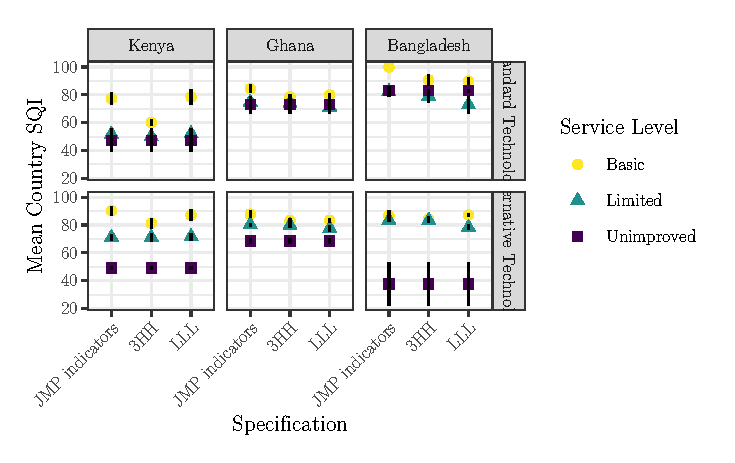
\includegraphics[width=0.99\linewidth]{figures/newlevels.eps}
    \caption{SQI distribution by service level specification}
    \label{fig:newlevels}
\end{figure}

Figure~\ref{fig:freqlevels} reports the changes in the relative frequency for each specification. Leaving the technology definition unaltered ("Standard technology") shows that lowering the threshold to three households ("JMP indicators" vs. "Expanded JMP") moves, as expected,  many shared facilities to the basic level. In Ghana and Bangladesh, applying the LLL specification (that does not take into consideration the number of households at all) increases the number of facilities classified as basic even more. In contrast, in Kenya, the LLL specification would decrease the share of sanitation facilities considered as basic, since few facilities are close to the household, have a light, and have a lock. Changing the definition of the technology requirements for a facility to be considered basic ("surrogate technology") has a very large impact on the frequency of facilities classified as unimproved and the consequences would strongly diverge for the three countries (see Figure~\ref{fig:freqlevels}, lower panel). In Kenya, the share of unimproved toilets would increase from 4\% to 85\%, in Ghana from 4\% to 45\%, and in Bangladesh decrease from 80\% to 1\%. This result also shows that the currently used technology threshold (or any other) has huge implications for whether we assume poor urban areas largely have adequate sanitation or not. 

\begin{figure}[ht]
    \centering
    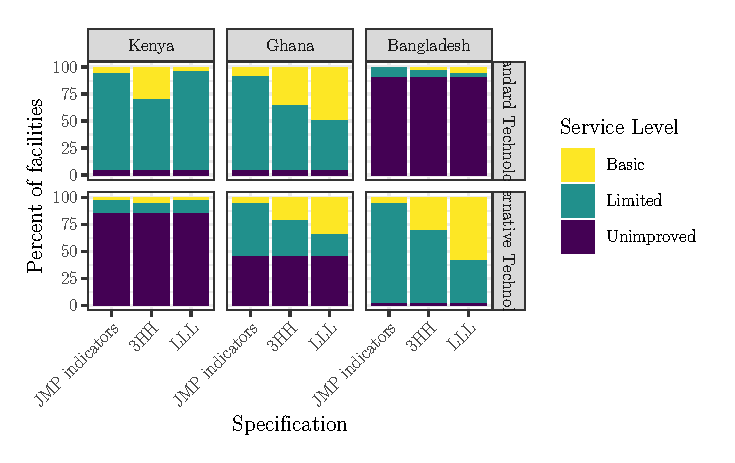
\includegraphics[width=0.99\linewidth]{figures/freqlevels.eps}
    \caption{SQI distribution by service level specification}
    \label{fig:freqlevels}
\end{figure}

\FloatBarrier

%%%%%%%%%%%%%%%%%%%%%%%%%%%%%%%%%%%%%%%%%%%%%%%%
% Conclusion
%%%%%%%%%%%%%%%%%%%%%%%%%%%%%%%%%%%%%%%%%%%%%%%%
\section{Conclusion}
\label{sec:conclusion}
In this paper, we developed a Sanitation Quality Indicator (SQI), a composite index measuring the observed cleanliness, safety, and privacy of sanitation facilities and analyzed its correlation with self-reported indicators of households’ toilets in cities of Kenya, Bangladesh and Ghana. The results indicate if and under what conditions shared sanitation facilities can be considered to be "adequate." Our results can also support the modification of the internationally applied JMP's sanitation service ladder for higher informative power. To do so, we suggest collecting additional information to assess the sanitation progress across countries through international applied household surveys, such as the Demographic and Health Surveys (DHS) and the Multiple Indicator Cluster Surveys.

Based on our results, the user interface technology, the number of sharing households, the toilets location, a door that is lockable from inside and outside, and lighting, are predictive indicators of sanitation quality. A cleaning rota and floor tiling is also weakly associated with higher sanitation quality. In contrast, a water source on the premises, gender-separated cubicles, the users' relationship, toilet age, a landlord living on the same plot, and a bin inside the cubicle are not correlated with sanitation quality. Second, we find that even though private toilets show a generally higher sanitation quality compared to shared toilets, the magnitude of the relationship varies considerably across countries. Toilets that are only shared by two and three households are mostly cleaner, safer, and more private than toilets shared by four or more households. Third, our results indicate that pit latrines with a slab show a considerably lower sanitation quality than toilets with flush or pour-flush technology. This is in contrast to JMP's classification, which makes no distinction between (pour-)flush facilities and pit latrines with a slab.

The JMP sanitation service levels constitute a classification system exclusively based on two dichotomous indicators, improved technology and shared facility, which are only partly informative as sanitation quality indicators. Classifying pit latrines as unimproved sanitation (with/without slab) leads to a considerable improvement in sanitation quality prediction relative to the current JMP sanitation service level specification. However, under this new specification, many more toilets would be classified as unimproved in poor urban areas. In contrast, increasing the number of households from one to three as a decisive criterion for basic sanitation or ignoring the number of households altogether and instead focusing on different indicators (location, lighting, lock) does not substantially affect the indicators’ predictive performance with regard to sanitation quality, but it strongly increases the share of toilets classified as basic. Such an adjustment, therefore, helps to focus scarce resources on the remaining "limited" category for a better targeting of future investments. 

Our results also show the large heterogeneity across poor urban settlements -- even though all were part of the (second) largest city in a middle-income country. The most commonly found sanitation technology varied considerably and the correlation of various indicators with sanitation quality was different across contexts. Toilets in Kumasi (Ghana) showed on average a higher sanitation quality than toilets in Kisumu (Kenya) and Dhaka (Bangladesh), even when controlling for all toilet characteristics. Hence, context seems to be particularly relevant for urban sanitation and research that analyzes these country-specific differences in more detail would shed more light contextual factors. Finally, exploring the causal mechanisms of the impact of the identified indicators and toilet quality would help to better inform future policy decisions. 


\clearpage

% BibTeX users please use one of
\bibliographystyle{spbasic}      % basic style, author-year citations

\bibliography{references.bib}   % name your BibTeX data base

% Appendix______________________________________________________________________
\clearpage
\appendix
\begin{landscape}
\section{Variable description}
\label{sec:variables}


\begin{longtable}{l l l l}
\caption{Variable description\label{tab:variables}}\\
\hline
Name &
  Values/Range &
  Description &
  \begin{tabular}[c]{@{}l@{}}Type \\ (observed/reported)\end{tabular} \\ \hline
\begin{tabular}[c]{@{}l@{}}Cleanliness \\ (observed/reported)\end{tabular} &
  \begin{tabular}[c]{@{}l@{}}Very dirty-Very clean\\ (5 levels)\end{tabular} &
  \begin{tabular}[c]{@{}l@{}}Cleanliness assessment of the toilet \\ cubicle by enumerators and respondents.\end{tabular} &
  observed/reported \\
 &
   &
   &
   \\
\begin{tabular}[c]{@{}l@{}}Toilet clean\\ (composite)\end{tabular} &
  Not clean/clean &
  \begin{tabular}[c]{@{}l@{}}Cleanliness assessment of the toilet cubicle \\ if at least one of the following is present:\\ visible feces, solid waste, insects.\end{tabular} &
  observed \\
 &
   &
   &
   \\
Visible feces &
  Yes/no &
  \begin{tabular}[c]{@{}l@{}}Visible feces inside the toilet cubicle\\ (on the floor or inside the pan).\end{tabular} &
  observed \\
 &
   &
   &
   \\
Solid waste &
  Yes/no &
  \begin{tabular}[c]{@{}l@{}}Solid waste inside the toilet cubicle \\ (toilet paper, cigarette butts, etc.).\end{tabular} &
  observed \\
 &
   &
   &
   \\
Insects &
  Yes/no &
  \begin{tabular}[c]{@{}l@{}}Substantial amount (not readily countable) \\ of insects inside the toilet cubicle.\end{tabular} &
  observed \\
 &
   &
   &
   \\
Toilet full or clogged &
  Yes/no &
  \begin{tabular}[c]{@{}l@{}}Visibly full pit (if latrine) or clogged \\ water seal (if flush/pour-flush).\end{tabular} &
  observed \\
 &
   &
   &
   \\
Wall material &
  high/low quality &
  \begin{tabular}[c]{@{}l@{}}At least a rudimentary wall without holes \\ that allow seeing through.\end{tabular} &
  observed \\
 &
   &
   &
   \\
Floor material &
  high/low quality &
  \begin{tabular}[c]{@{}l@{}}At least a finished floor without cracks/\\ holes in the slab.\end{tabular} &
  observed \\
 &
   &
   &
   \\
Roof material &
  high/low quality &
  \begin{tabular}[c]{@{}l@{}}At least natural roofing without holes that\\ allow rainwater to enter the cubicle.\end{tabular} &
  observed \\
 &
   &
   &
   \\
\begin{tabular}[c]{@{}l@{}}Handwashing station \\ (with soap)\end{tabular} &
  Yes/no &
  \begin{tabular}[c]{@{}l@{}}Handwashing facility with water and soap\\ within 5m of the toilet facility.\end{tabular} &
  observed \\
 &
   &
   &
   \\
Toilet technology &
  \begin{tabular}[c]{@{}l@{}}Flush to sewer/septic/pit\\ Flush to elsewhere\\ Pit latrine (with slab)\\ Pit latrine (no slab)/other\end{tabular} &
  \begin{tabular}[c]{@{}l@{}}According to the definition provided by\\ \cite{JMP2018}. If the respondent could not\\ determine the outflow or when it drained\\ into the open, it was categorized as\\  "to elsewhere".\end{tabular} &
  reported \\
Sharing HHs &
  1 HH-more than 10 HH &
  \begin{tabular}[c]{@{}l@{}}Number of HHs sharing the same cubicle\\ including the respondent's HH.\end{tabular} &
  reported \\
 &
   &
   &
   \\
Location &
  \begin{tabular}[c]{@{}l@{}}Inside dwelling,\\ Inside compound/on plot\\ Elsewhere\end{tabular} &
  \begin{tabular}[c]{@{}l@{}}The toilet's location. If not inside a structurally\\ delimited plot or compound or more than 30m\\ from the respondent's dwelling, it was \\ categorized as "Elsewhere".\end{tabular} &
  reported \\
 &
   &
   &
   \\
\begin{tabular}[c]{@{}l@{}}Improved water\\ on premises\end{tabular} &
  Yes/No &
  \begin{tabular}[c]{@{}l@{}}Improved water source according to the\\ definition provided by \cite{JMP2018}\\ inside the dwelling, plot, or compound.\end{tabular} &
  reported \\
 &
   &
   &
   \\
Lighting &
  Yes/No &
  Functional nightlight inside the cubicle. &
  reported \\
 &
   &
   &
   \\
Lockable door &
  \begin{tabular}[c]{@{}l@{}}No lockable door\\ Only inside\\ Only outside\\ Outside and inside\end{tabular} &
  Lockable door from the inside outside or both. &
  reported \\
 &
   &
   &
   \\
Tiling &
  Yes/no &
  Ceramic tiles on the floor. &
  reported \\
 &
   &
   &
   \\
Gender separated &
  Yes/no &
  Gender separated cubicles. &
  reported \\
 &
   &
   &
   \\
Cleaning rota &
  Yes/no &
  \begin{tabular}[c]{@{}l@{}}Reported use of c rota to organize cleaning \\ duties.\end{tabular} &
  reported \\
 &
   &
   &
   \\
User relationship &
  \begin{tabular}[c]{@{}l@{}}Only relatives\\ Close neighbors/landlord\\ Other tenants/unknown\end{tabular} &
  \begin{tabular}[c]{@{}l@{}}Degree of user relationship between all sharing\\ HHs. Only relatives also refers to extended \\ family. Close neighbors are known by name\\ and require regular social interaction.\end{tabular} &
  reported \\
 &
   &
   &
   \\
Age of toilet &
  Years &
  \begin{tabular}[c]{@{}l@{}}Age of the toilet structure in years. If the toilet\\ was already existing when the respondent \\ moved in, categorized as "More than 9 years / \\ don't know".\end{tabular} &
  reported \\
 &
   &
   &
   \\
Landlord on plot &
  Yes/no &
  \begin{tabular}[c]{@{}l@{}}Landlord or caretaker living on the same plot\\ as the respondent. "Yes", if the respondent is \\ the landlord.\end{tabular} &
  reported \\
 &
   &
   &
   \\
Bin inside cubicle &
  Yes/no &
  \begin{tabular}[c]{@{}l@{}}Waste bin for toilet paper or MHM materials\\ inside the toilet cubicle.\end{tabular} &
  reported \\ \hline
\end{longtable}

\end{landscape}
\section{Construction of the SQI}
\label{sec:sqi}
Formally, the SQI was defined as follows. Let $k=(1,2,\dots,K)$ be the number of variables included in the index, $j=(1,2,\dots,J_k)$ the number of categories in each variable $k$ and $f=(1,2,\dots,N)$ the number of toilet facilities. The binary indicator $I$ represents the occurrence of a category $j$. Then the SQI is calculated as
\begin{equation}
\label{eq:sqi}
    SQI_f = \frac{1}{K} \sum_{k=1}^{K} \sum_{j=1}^{J_k} W_{jk} I_{fjk}
\end{equation}
with the weight assigned to each category $j$ of each variable $k$ determined by
\begin{equation}
    W_{jk} = \frac{s_k - s_{min}}{\sqrt{\lambda_1}},
\end{equation}
where $s_jk$ denotes a vector of coordinates of the first dimension (the first principal component) given by MCA (also referred to as factor scores), and $\lambda_1$ is the eigenvalue associated with the first principal component. Therefore, the weights applied to each component of the index are normalized by the lowest factor score and the square root of the eigenvalue in order to ensure that the lowest index score is zero and all other index scores are positive. Following equation~\ref{eq:sqi}, the SQI is therefore simply an average of the weighted sum of each quality variable's observed presence. 

The SQI is normalized to facilitate the interpretation of marginal effects:
\begin{equation}
\label{eq:sqi_norm}
    SQI_f^{norm} = \frac{SQI_f - min(SQI)}{max(SQI)-min(SQI)} \times 100.
\end{equation}
As a result of equation~\ref{eq:sqi_norm}, the SQI can exhibit values between 0 and 100, with a score of 100 indicating that a toilet meets all quality requirements as defined by the outcome variables presented in section~\ref{sec:measures}.

\section{MCA results}

\begin{figure}[ht]
    \centering
    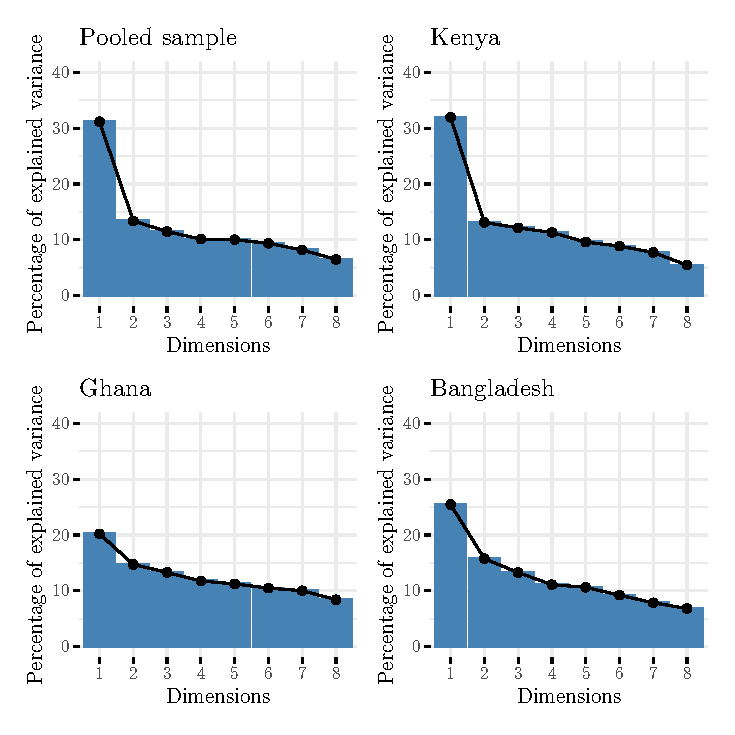
\includegraphics{figures/scree_pooled.eps}
    \caption{Screeplots of explained variance in MCA}
    \label{fig:scree}
\end{figure}

As a result of the MCA, we obtain a number of principal components (PC). The MCA sets the weights of the the first PC in order to capture as much of the total variance as possible, while being as uncorrelated as possible to the other PCs. Figure~\ref{fig:scree} shows how much of the total variance in our data is explained by each PC. The top-left panel shows that the first PC captures 31.2\% of the total variance, followed by 13.4\% in the second PC. In Kenya (top-right panel), the first PC explains a similarly large percentage of the variance as in the pooled sample (31.9\%). In Bangladesh (25.5\%; bottom-right) and in Ghana (20.2\%; bottom-left), the percentages are smaller. 

Table~\ref{tab:weights} shows the statistical weights $W_{jk}$ resulting from the MCA for the pooled analysis ("Overall") and by country. In all cases, the positive feature (e.g., the absence of visible feces or high quality floor material) has higher scores compared to the negative feature (e.g., the presence of visible feces or low quality floor material). At the same time, the results show considerable variation across countries (cities).
\begin{table}[ht]

\caption{\label{tab:weights}Statistical weights for the construction of the SQI}
\centering
\begin{tabular}[t]{lcccc}
\toprule
Variable & Overall & Kenya & Ghana & Bangladesh\\
\midrule
Visible feces: yes & 0.80 & 0.54 & 0.00 & 1.86\\
Visible feces: no & 3.70 & 3.12 & 4.77 & 4.54\\
Insects: yes & 1.81 & 1.50 & 2.54 & 2.88\\
Insects: no & 3.96 & 3.86 & 4.86 & 4.53\\
Solid waste: yes & 1.58 & 0.99 & 2.01 & 2.24\\
Solid waste: no & 3.74 & 3.06 & 5.03 & 4.77\\
Floor material: low quality & 0.00 & 0.16 & 0.10 & 0.00\\
Floor material: high quality & 3.35 & 2.58 & 4.50 & 4.26\\
Roof material: low quality & 1.12 & 0.90 & 2.05 & 1.71\\
Roof material: high quality & 3.57 & 2.88 & 4.63 & 4.46\\
Wall material: low quality & 0.31 & 0.00 & 1.48 & 0.35\\
Wall material: high quality & 3.40 & 2.59 & 4.51 & 4.51\\
Toilet full/clogged: yes & 0.41 & 0.54 & 0.18 & 0.64\\
Toilet full/clogged: no & 3.56 & 3.02 & 4.77 & 4.18\\
Handwashing station with soap: no & 2.90 & 2.11 & 4.09 & 3.88\\
Handwashing station with soap: yes & 4.22 & 5.77 & 7.05 & 4.31\\
\bottomrule
\end{tabular}
\end{table}

\section{Observed versus reported sanitation quality} 
\label{sec:reliability}
As discussed in Section~\ref{sec:measures}, we found that asking households about their toilet’s sanitation quality leads to high measurement error -- probably because of social desirability bias. Figure~\ref{fig:reliability} illustrates this point by showing the cleanliness assessment (one of the three dimensions of the SQI) from different data sources.

\begin{figure}[htbp]
    \centering
    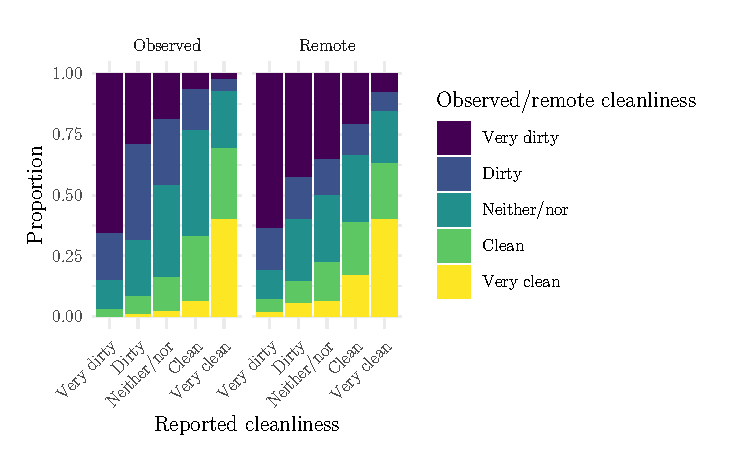
\includegraphics[width=0.8\textwidth]{figures/reliability.eps}
    \caption{Reliability of cleanliness assessments}
    \label{fig:reliability}
\end{figure}

Figure~\ref{fig:reliability} shows the distribution of toilet cleanliness ratings based on respondent-reported data compared to observed data recorded by enumerators during spot-checks and compared to a remote coding of photographs taken during the spot-checks. The reported data represents the respondents' subjective assessment of the toilets' general cleanliness on a five-point Likert scale. The observed data was collected by enumerators after the interviews, also using a five-point Likert scale. Enumerators paid special attention to visible feces, insects, solid waste, as well as spilled urine and other bodily substances. Third,  enumerators took photos of the toilets (from outside and within) during the spot-checks that were later rated by research assistants who were otherwise not involved in this study. The left panel shows the comparison between reported and observed data, while the right panel shows the comparison between reported and remotely-coded data.

Each bar shows the distribution of observed (by enumerators) or remotely-coded (by research assistants) cleanliness ratings for a self-reported cleanliness level. For example, the first bar contains all toilet cubicles that were considered very dirty by their users. About 60\% of these cubicles were also considered to be very dirty by the enumerators. The graph shows that even if there is a positive correlation between reported, observed, and remote assessments, there is considerable disagreement between households and the other two types of observers. In general, households report their toilets to be cleaner than external observers. Whereas households only reported 11\% of toilets to be dirty or very dirty, the data based on observations suggest that 26\% of the shared toilets are dirty or very dirty. These results show that self-reported sanitation quality is not a reliable indicator of observed quality.


\section{Robustness of the SQI}
\label{sec:robustness}
\begin{figure}[ht]
    \centering
    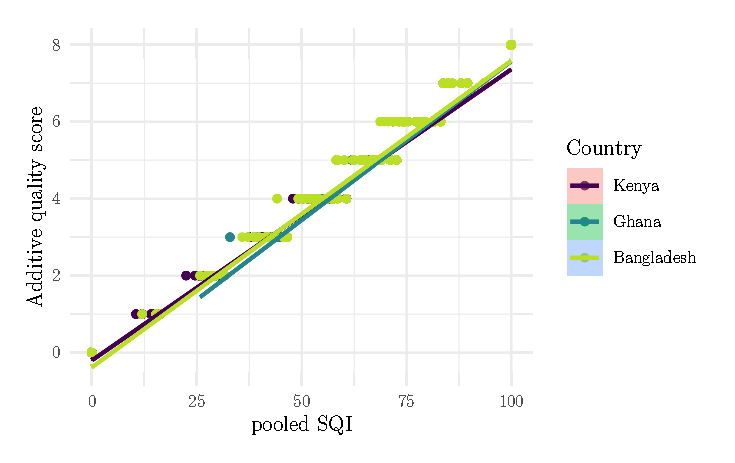
\includegraphics[width=0.8\textwidth]{figures/cor_additive.eps}
    \caption{Correlation of additive quality score and SQI}
    \label{fig:corr_additive}
\end{figure}


\begin{center}
\begin{footnotesize}
\begin{ThreePartTable}
\begin{TableNotes}[flushleft]
\tiny{\item[\hspace{-5mm}] Standard errors are clustered on the compound level. \item[\hspace{-5mm}] Pooled regression includes country fixed effects. \item[\hspace{-5mm}] $^{***}p<0.001$; $^{**}p<0.01$; $^{*}p<0.05$.}
\end{TableNotes}
\begin{longtable}{l@{} c@{} c@{} c@{} c@{}}
\caption{OLS regression results of additive SQI on indicators}
\label{tab:reg_add_ctry}\\
\toprule
 & \multicolumn{4}{c}{Additive SQI} \\
\cmidrule(lr){2-5}
 & All & Kenya & Ghana & Bangladesh \\
\midrule
\endfirsthead
\toprule
 & \multicolumn{4}{c}{Additive SQI} \\
\cmidrule(lr){2-5}
 & All & Kenya & Ghana & Bangladesh \\
\midrule
\endhead
\bottomrule
\endfoot
\bottomrule
\insertTableNotes\\
\endlastfoot
Technology (ref=\textit{Flush})                            &               &               &               &              \\
                                                           &               &               &               &              \\
\quad Pit latrine (with slab)                              & $-0.85^{***}$ & $-1.16^{***}$ & $-0.22$       &              \\
                                                           & $(0.18)$      & $(0.23)$      & $(0.29)$      &              \\
\quad Pit latrine (no slab)/other                          & $-1.28^{***}$ & $-2.45^{***}$ & $0.11$        & $-1.89^{*}$  \\
                                                           & $(0.29)$      & $(0.46)$      & $(0.31)$      & $(0.90)$     \\
Outflow (ref=\textit{Piped sewer/septic tank})             &               &               &               &              \\
                                                           &               &               &               &              \\
\quad Pit                                                  & $-0.14$       & $-0.55^{*}$   & $-0.51$       & $-0.77$      \\
                                                           & $(0.18)$      & $(0.25)$      & $(0.29)$      & $(0.55)$     \\
\quad Elsewhere                                            & $0.06$        & $-0.11$       & $-0.49$       & $-0.31^{*}$  \\
                                                           & $(0.13)$      & $(0.23)$      & $(0.38)$      & $(0.13)$     \\
Sharing HHs (ref=\textit{1 HH})                            &               &               &               &              \\
                                                           &               &               &               &              \\
\quad 2 HH                                                 & $-0.34^{*}$   & $-0.45$       & $0.09$        & $-0.99^{*}$  \\
                                                           & $(0.15)$      & $(0.26)$      & $(0.15)$      & $(0.50)$     \\
\quad 3 HH                                                 & $-0.35^{*}$   & $-0.46$       & $-0.10$       & $-0.72$      \\
                                                           & $(0.15)$      & $(0.27)$      & $(0.16)$      & $(0.52)$     \\
\quad 4 HH                                                 & $-0.60^{***}$ & $-0.82^{**}$  & $-0.07$       & $-1.06^{*}$  \\
                                                           & $(0.15)$      & $(0.27)$      & $(0.16)$      & $(0.53)$     \\
\quad 5 HH                                                 & $-0.63^{***}$ & $-0.89^{**}$  & $-0.18$       & $-0.85$      \\
                                                           & $(0.15)$      & $(0.29)$      & $(0.15)$      & $(0.52)$     \\
\quad 6 HH                                                 & $-0.62^{***}$ & $-0.87^{**}$  & $-0.20$       & $-0.97$      \\
                                                           & $(0.16)$      & $(0.31)$      & $(0.16)$      & $(0.52)$     \\
\quad 7 HH                                                 & $-0.51^{**}$  & $-0.55^{*}$   & $-0.19$       & $-0.91$      \\
                                                           & $(0.16)$      & $(0.28)$      & $(0.20)$      & $(0.52)$     \\
\quad 8 HH                                                 & $-0.66^{***}$ & $-1.06^{***}$ & $-0.03$       & $-0.82$      \\
                                                           & $(0.17)$      & $(0.32)$      & $(0.19)$      & $(0.52)$     \\
\quad 9 HH                                                 & $-0.63^{***}$ & $-0.84^{*}$   & $-0.14$       & $-1.04$      \\
                                                           & $(0.19)$      & $(0.33)$      & $(0.22)$      & $(0.54)$     \\
\quad 10 HH                                                & $-0.82^{***}$ & $-1.03^{**}$  & $-0.24$       & $-1.36^{*}$  \\
                                                           & $(0.19)$      & $(0.35)$      & $(0.22)$      & $(0.55)$     \\
\quad $>$10 HH                                             & $-0.90^{***}$ & $-1.31^{***}$ & $-0.27$       & $-1.13^{*}$  \\
                                                           & $(0.15)$      & $(0.25)$      & $(0.18)$      & $(0.51)$     \\
Location (ref=\textit{Inside dwelling})                    &               &               &               &              \\
                                                           &               &               &               &              \\
\quad Inside compound                                      & $-0.26^{*}$   & $0.11$        & $-0.52^{***}$ & $0.17$       \\
                                                           & $(0.11)$      & $(0.26)$      & $(0.10)$      & $(0.30)$     \\
\quad Outside compound                                     & $-1.02^{***}$ & $-0.62$       & $-0.63^{**}$  & $-0.86$      \\
                                                           & $(0.20)$      & $(0.33)$      & $(0.22)$      & $(0.49)$     \\
Water on premises (ref=\textit{No})                        & $0.14$        & $0.24^{*}$    & $-0.04$       & $0.29$       \\
                                                           & $(0.08)$      & $(0.12)$      & $(0.08)$      & $(0.31)$     \\
Lighting (ref=\textit{No})                                 & $0.34^{***}$  & $0.13$        & $0.28^{***}$  & $0.46^{***}$ \\
                                                           & $(0.07)$      & $(0.23)$      & $(0.08)$      & $(0.11)$     \\
Lockable door (ref=\textit{Not lockable})                  &               &               &               &              \\
                                                           &               &               &               &              \\
\quad Only inside                                          & $0.72^{***}$  & $0.82^{**}$   & $-0.05$       & $0.99^{**}$  \\
                                                           & $(0.14)$      & $(0.29)$      & $(0.19)$      & $(0.34)$     \\
\quad Only outside                                         & $0.73^{***}$  & $0.89^{***}$  & $-0.08$       & $0.42$       \\
                                                           & $(0.15)$      & $(0.20)$      & $(0.17)$      & $(0.66)$     \\
\quad Outside and inside                                   & $1.20^{***}$  & $1.44^{***}$  & $0.12$        & $1.45^{***}$ \\
                                                           & $(0.11)$      & $(0.16)$      & $(0.12)$      & $(0.32)$     \\
Tiling (ref=\textit{No})                                   & $0.37^{***}$  & $0.48^{**}$   & $0.35^{***}$  & $0.35$       \\
                                                           & $(0.07)$      & $(0.17)$      & $(0.08)$      & $(0.19)$     \\
Gender separated (ref=\textit{No})                         & $0.13$        & $0.17$        & $0.14$        & $-0.05$      \\
                                                           & $(0.14)$      & $(0.64)$      & $(0.16)$      & $(0.26)$     \\
Cleaning rota (ref=\textit{No})                            & $0.31^{***}$  & $0.21$        & $0.12$        & $0.33^{**}$  \\
                                                           & $(0.07)$      & $(0.16)$      & $(0.08)$      & $(0.12)$     \\
User relationship (ref=\textit{Relatives/close neighbors}) &               &               &               &              \\
                                                           &               &               &               &              \\
\quad Other tenants/unknown                                & $-0.22^{*}$   & $-0.33^{*}$   & $-0.19^{*}$   & $-0.05$      \\
                                                           & $(0.09)$      & $(0.14)$      & $(0.09)$      & $(0.37)$     \\
Toilet age, years (ref=\textit{$<$1})                      &               &               &               &              \\
                                                           &               &               &               &              \\
\quad 1-3                                                  & $-0.04$       & $0.07$        & $0.06$        & $-0.15$      \\
                                                           & $(0.09)$      & $(0.14)$      & $(0.16)$      & $(0.13)$     \\
\quad 4-6                                                  & $0.04$        & $0.09$        & $0.16$        & $-0.07$      \\
                                                           & $(0.10)$      & $(0.15)$      & $(0.17)$      & $(0.15)$     \\
\quad 7-9                                                  & $-0.02$       & $-0.24$       & $0.42^{*}$    & $-0.08$      \\
                                                           & $(0.12)$      & $(0.22)$      & $(0.17)$      & $(0.20)$     \\
\quad $>$9                                                 & $-0.14$       & $-0.25$       & $0.12$        & $-0.19$      \\
                                                           & $(0.09)$      & $(0.16)$      & $(0.16)$      & $(0.13)$     \\
Landlord on plot (ref=\textit{No})                         & $-0.06$       & $-0.11$       & $0.03$        & $0.02$       \\
                                                           & $(0.07)$      & $(0.11)$      & $(0.11)$      & $(0.11)$     \\
Bin inside cubicle (ref=\textit{No})                       & $-0.12^{*}$   & $0.17$        & $-0.10^{*}$   & $0.22$       \\
                                                           & $(0.05)$      & $(0.17)$      & $(0.05)$      & $(0.25)$     \\
Ghana FE                                                   & $0.80^{***}$  &               &               &              \\
                                                           & $(0.10)$      &               &               &              \\
Bangladesh FE                                              & $-0.05$       &               &               &              \\
                                                           & $(0.16)$      &               &               &              \\
(Intercept)                                                & $5.48^{***}$  & $5.91^{***}$  & $6.82^{***}$  & $5.14^{***}$ \\
                                                           & $(0.18)$      & $(0.32)$      & $(0.24)$      & $(0.50)$     \\
\midrule
R$^2$                                                      & $0.42$        & $0.39$        & $0.29$        & $0.24$       \\
Adj. R$^2$                                                 & $0.42$        & $0.37$        & $0.27$        & $0.22$       \\
Num. obs.                                                  & $3600$        & $1229$        & $1087$        & $1284$       \\
N Clusters                                                 & $2013$        & $687$         & $633$         & $693$        \\
\end{longtable}
\end{ThreePartTable}
\end{footnotesize}
\end{center}

\FloatBarrier

\section{Quality indicators within the JMP Framework: additional results}
\label{sec:newlevelsapp}
\begin{table}[ht]

\caption{\label{tab:newlevels}Mean SQI and frequency by sanitation level specification}
\centering
\resizebox{\linewidth}{!}{
\begin{tabular}[t]{lcccccc}
\toprule
\multicolumn{1}{c}{ } & \multicolumn{2}{c}{Kenya} & \multicolumn{2}{c}{Ghana} & \multicolumn{2}{c}{Bangladesh} \\
\cmidrule(l{3pt}r{3pt}){2-3} \cmidrule(l{3pt}r{3pt}){4-5} \cmidrule(l{3pt}r{3pt}){6-7}
Level specification & Standard Technology & Alternative Technology & Standard Technology & Alternative Technology & Standard Technology & Alternative Technology\\
\midrule
\addlinespace[0.3em]
\multicolumn{7}{l}{\textbf{JMP indicators}}\\
\hspace{1em}Basic & 85.9 (6\%) & 95.9 (3\%) & 91.2 (9\%) & 93.8 (6\%) & 100 (0\%) & 86.4 (6\%)\\
\hspace{1em}Limited & 60.8 (90\%) & 82 (11\%) & 84.5 (87\%) & 88.9 (49\%) & 78.3 (10\%) & 79.4 (93\%)\\
\hspace{1em}Unimproved & 54.5 (4\%) & 58.1 (85\%) & 83.3 (4\%) & 79.7 (45\%) & 79.4 (90\%) & 35.1 \vphantom{2} (1\%)\\
\addlinespace[0.3em]
\multicolumn{7}{l}{\textbf{Expanded JMP (3HH)}}\\
\hspace{1em}Basic & 69.4 (30\%) & 89 (6\%) & 87.1 (36\%) & 90.6 (22\%) & 87.5 (3\%) & 81.4 (31\%)\\
\hspace{1em}Limited & 59.1 (66\%) & 82.4 (9\%) & 84 (60\%) & 88.7 (33\%) & 74.7 (7\%) & 79.1 (68\%)\\
\hspace{1em}Unimproved & 54.5 (4\%) & 58.1 (85\%) & 83.3 (4\%) & 79.7 (45\%) & 79.4 (90\%) & 35.1 \vphantom{1} (1\%)\\
\addlinespace[0.3em]
\multicolumn{7}{l}{\textbf{Location + Lock + Lighting (LLL)}}\\
\hspace{1em}Basic & 85.9 (4\%) & 93.5 (3\%) & 88.3 (49\%) & 90.8 (34\%) & 86.4 (6\%) & 83.6 (58\%)\\
\hspace{1em}Limited & 61.2 (92\%) & 82.5 (11\%) & 81.9 (47\%) & 87.2 (21\%) & 68.3 (4\%) & 74.4 (40\%)\\
\hspace{1em}Unimproved & 54.5 (4\%) & 58.1 (85\%) & 83.3 (4\%) & 79.7 (45\%) & 79.4 (90\%) & 35.1 (1\%)\\
\bottomrule
\end{tabular}}
\end{table}

\end{document}
% end of file template.tex


